\documentclass[10pt]{article}
\usepackage[english]{babel}
\usepackage[utf8]{inputenc}

% includes references in the table of contents
\usepackage[nottoc]{tocbibind}

\usepackage{amsthm}
\theoremstyle{plain}
\usepackage{thmtools}
\usepackage{enumerate}
\newtheorem{theorem}{Theorem}

\theoremstyle{definition}
\newtheorem{definition}[theorem]{Definition}

\usepackage{algorithm}
\usepackage{algpseudocode}

% Algorithmic modifications
\makeatletter
\newcommand{\algorithmicbreak}{\textbf{break}}
\newcommand{\Break}{\State \algorithmicbreak}

\algnewcommand\AND{\textbf{and }}
\algnewcommand\OR{\textbf{or }}
\algnewcommand\NOT{\textbf{not }}

\newenvironment{breakablealgorithm}
  {% \begin{breakablealgorithm}
   \begin{center}
     \refstepcounter{algorithm}% New algorithm
     \hrule height.8pt depth0pt \kern2pt% \@fs@pre for \@fs@ruled
     \renewcommand{\caption}[2][\relax]{% Make a new \caption
       {\raggedright\textbf{\fname@algorithm~\thealgorithm} ##2\par}%
       \ifx\relax##1\relax % #1 is \relax
         \addcontentsline{loa}{algorithm}{\protect\numberline{\thealgorithm}##2}%
       \else % #1 is not \relax
         \addcontentsline{loa}{algorithm}{\protect\numberline{\thealgorithm}##1}%
       \fi
       \kern2pt\hrule\kern2pt
     }
  }{% \end{breakablealgorithm}
     \kern2pt\hrule\relax% \@fs@post for \@fs@ruled
   \end{center}
  }
\makeatother

\usepackage{booktabs}
\usepackage{hyperref}
\usepackage{amsmath}
\usepackage{amssymb}
\usepackage{graphicx}
\usepackage{subcaption}
\usepackage{fancyhdr}
\usepackage{vmargin}
\setmarginsrb{2cm}  % left margin
             {2cm}  % top margin
             {2cm}  % right margin
             {2cm}  % bottom margin
             {1.5cm}  % head height
             {1cm}  % head sep
             {1.5cm}  % foot height
             {1cm}  % foot sep
   
\title{Support Vector Machines}
\author{Donato Meoli}
\date{March, 2021}

\makeatletter
\let\thetitle\@title
\let\theauthor\@author
\let\thedate\@date
\makeatother

\pagestyle{fancy}
\fancyhf{}
\rhead{\thepage}
\lhead{\thetitle}
\cfoot{}

\begin{document}

\begin{titlepage}
	\centering
    \vspace*{0.5 cm}
    
\includegraphics[scale=0.5]{img/unipi.png}\\[1.0 cm]
    \textsc{\LARGE University of Pisa}\\[0.5 cm]
    \textsc{\Large Department of Computer Science}\\[1.5 cm]
	\textsc{\large Computational Mathematics \\ Wildcard Project nr. 5 with Machine Learning \\ Group 35}\\[0.5 cm]
	\rule{\linewidth}{0.2 mm} \\[0.4 cm]
	{ \huge \bfseries \thetitle}\\
	\rule{\linewidth}{0.2 mm} \\[1.5 cm]
	\centering \textsc{\large \emph{Author:}}\\[0.5 cm]
	\begin{minipage}{0.4\textwidth}
		\begin{center} \large
			\textbf{\theauthor}
			\texttt{\href{mailto::d.meoli@studenti.unipi.it}{d.meoli@studenti.unipi.it}}
		\end{center}
		\end{minipage}~
		\begin{minipage}{0.4\textwidth}
	\end{minipage}\\[2 cm]
	{\large \thedate}\\[2 cm]
	\vfill
\end{titlepage}

\tableofcontents

\pagebreak

\listoffigures

\pagebreak

\listoftables

\pagebreak

\listofalgorithms
\addcontentsline{toc}{section}{List of Algorithms}

\pagebreak

\listoftheorems

\pagebreak

\section{Track}

\begin{itemize}
\item[\texttt{(M1.1)}] is a \emph{Support Vector Classifier (SVC)} with the \emph{hinge} loss.

\begin{itemize}
\item[\texttt{(A1.1.1)}] is the \emph{AdaGrad} algorithm \cite{duchi2011adaptive}, a \emph{deflected subgradient} method for solving the SVC in its \emph{primal} formulation.

\item[\texttt{(A1.1.2)}] is the \emph{Sequential Minimal Optimization (SMO)} algorithm \cite{platt1998sequential} (see \cite{keerthi2001improvements} for improvements), an ad hoc \emph{active set} method for training a SVC in its \emph{Wolfe dual} formulation with \emph{linear}, \emph{polynomial} and \emph{gaussian} kernels.

\item[\texttt{(A1.1.3)}] is the \emph{AdaGrad} algorithm \cite{duchi2011adaptive}, a \emph{deflected subgradient} method for solving the SVC in its \emph{Lagrangian dual} formulation with \emph{linear}, \emph{polynomial} and \emph{gaussian} kernels.
\end{itemize}

\end{itemize}

\begin{itemize}
\item[\texttt{(M1.2)}] is a \emph{Support Vector Classifier (SVC)} with the \emph{squared hinge} loss.

\begin{itemize}
\item[\texttt{(A1.2.1)}] is standard \emph{gradient descent} approach for solving the SVC in its \emph{primal} formulation.
\end{itemize}

\end{itemize}

\bigskip

\begin{itemize}
\item[\texttt{(M2.1)}] is a \emph{Support Vector Regression (SVR)} with the \emph{epsilon-insensitive} loss.

\begin{itemize}
\item[\texttt{(A2.1.1)}] is the \emph{AdaGrad} algorithm \cite{duchi2011adaptive}, a \emph{deflected subgradient} method for solving the SVR in its \emph{primal} formulation.

\item[\texttt{(A2.1.2)}] is the \emph{Sequential Minimal Optimization (SMO)} algorithm \cite{flake2002efficient} (see \cite{shevade1999improvements} for improvements), an ad hoc \emph{active set} method for training a SVR in its \emph{Wolfe dual} formulation with \emph{linear}, \emph{polynomial} and \emph{gaussian} kernels.

\item[\texttt{(A2.1.3)}] is the \emph{AdaGrad} algorithm \cite{duchi2011adaptive}, a \emph{deflected subgradient} method for solving the SVR in its \emph{Lagrangian dual} formulation with \emph{linear}, \emph{polynomial} and \emph{gaussian} kernels.
\end{itemize}

\end{itemize}

\begin{itemize}
\item[\texttt{(M2.2)}] is a \emph{Support Vector Regression (SVR)} with the \emph{squared epsilon-insensitive} loss.

\begin{itemize}
\item[\texttt{(A2.2.1)}] is a standard \emph{gradient descent} approach for solving the SVR in its \emph{primal} formulation.
\end{itemize}

\end{itemize}
\section{Abstract}

A \emph{Support Vector Machine} is a learning model used both for \emph{classification} and \emph{regression} tasks whose goal is to constructs a \emph{maximum margin separator}, i.e., a decision boundary with the largest distance from the nearest training data points.

The aim of this report is to compare the \emph{primal}, the \emph{Wolfe dual} \cite{fletcher2009support} and the \emph{Lagrangian dual} formulations of this model in terms of \emph{numerical precision}, \emph{accuracy} and \emph{complexity}.

Firstly, I will provide a detailed mathematical derivation of the model for all these formulations, then I will propose two algorithms to solve the optimization problem in case of \emph{constrained} or \emph{unconstrained} formulation of the problem, explaining their theoretical properties, i.e., \emph{convergence} and \emph{complexity}.

Finally, I will show some experiments for \emph{linearly} and \emph{nonlinearly} separable generated datasets to compare the performace of different \emph{kernels}, also by comparing the \emph{custom} results with \emph{sklearn} SVM implementations, i.e., \emph{liblinear} \cite{fan2008liblinear} and \emph{libsvm} \cite{chang2011libsvm} implementations, and \emph{cvxopt} \cite{vandenberghe2010cvxopt} QP solver.


\pagebreak

\section{Linear Support Vector Classifier}

Given $n$ training points, where each input $x_i$ has $m$ attributes, i.e., is of dimensionality $m$, and is in one of two classes $y_i=\pm1$, i.e., our training data is of the form:

\begin{equation}
	\{(x_i,y_i), x_i\in\Re^{m}, y_i=\pm1, i=1, \dots, n\} \label{eq:svc_data}
\end{equation}

For simplicity we first assume that data are (not fully) linearly separable in the input space $x$, meaning that we can draw a line separating the two classes when $m=2$, a plane for $m=3$ and, more in general, a hyperplane for an arbitrary $m$.

Support vectors are the examples closest to the separating hyperplane and the aim of support vector machines is to orientate this hyperplane in such a way as to be as far as possible from the closest members of both classes, i.e., we need to maximize this margin.

This hyperplane is represented by the equation $w^T x + b=0$. So, we need to find $w$ and $b$ so that our training data can be described by:

\begin{equation} \label{eq:svc_consts}
	\begin{aligned}
		& w^T x_i + b \geq +1 - \xi_i, \forall y_i=+1 \\
    	& w^T x_i + b \leq -1 + \xi_i, \forall y_i=-1 \\
    	& \xi_i \geq 0 \ \forall_i
	\end{aligned}
\end{equation}

where the positive slack variables $\xi_i$ are introduced to allow missclassified points. In this way data points on the incorrect side of the margin boundary will have a penalty that increases with the distance from it.

These two equations can be combined into:

\begin{equation} \label{eq:svc_const}
	\begin{aligned}
    	& y_i (w^T x_i + b) \geq 1 - \xi_i \ \forall_i \\
    	& \xi_i\geq 0 \ \forall_i
    \end{aligned}
\end{equation}

The margin is equal to $\displaystyle \frac{1}{\Vert w\Vert}$ and maximizing it subject to the constraint in \ref{eq:svc_const} while as we are trying to reduce the number of misclassifications is equivalent to finding:

\begin{equation} \label{eq:svc_obj}
    \begin{aligned}
        \min_{w,b,\xi} \quad & \Vert w \Vert + C \sum_{i=1}^{n} \xi_i \\
            \textrm{subject to} \quad & y_i (w^T x_i + b) \geq 1 - \xi_i \ \forall_i \\ & \xi_i \geq 0 \ \forall_i
    \end{aligned}
\end{equation}

Minimizing $\Vert w\Vert$ is equivalent to minimizing $\displaystyle \frac{1}{2}\Vert w\Vert^{2}$, but in this form we will deal with a convex optimization problem that has more desirable convergence properties. So we need to find:

\begin{equation} \label{eq:quad_svc_obj}
    \begin{aligned}
        \min_{w,b,\xi} \quad & \frac{1}{2} \Vert w \Vert^2 + C \sum_{i=1}^{n} \xi_i \\
            \textrm{subject to} \quad & y_i (w^T x_i + b) \geq 1 - \xi_i \ \forall_i \\ & \xi_i \geq 0 \ \forall_i
    \end{aligned}
\end{equation}

where the parameter $C$ controls the trade-off between the slack variable penalty and the size of the margin.

\begin{figure}[h!]
	\centering
	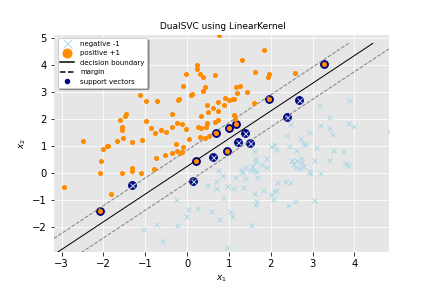
\includegraphics[scale=0.6]{img/linear_dual_svc_hyperplane.png}
	\caption{Linear SVC hyperplane}
	\label{fig:linear_dual_svc_hyperplane}
\end{figure}

\subsection{Primal Formulations}

The general primal unconstrained formulation takes the form:

\begin{equation} \label{eq:primal_svc}
    \min_{w,b} \mathcal{R}(w,b) + C \sum_{i=1}^n \mathcal{L}(w,b;x_i,y_i)
\end{equation}

where $\mathcal{R}(w, b)$ is the \emph{regularization term} and $\mathcal{L}(w,b;x_i,y_i)$ is the \emph{loss function} associated with the observation $(x_i,y_i)$.

\subsubsection{Hinge loss}

The quadratic optimization problem \ref{eq:quad_svc_obj} can be equivalently formulated as: 

\begin{equation} \label{eq:svc_hinge}
    \min_{w,b} \frac{1}{2} \Vert w \Vert^2 + C \sum_{i=1}^n \max(0, 1 - y_i (w^T x_i + b))
\end{equation}

where we make use of the \emph{hinge} loss defined as:

\begin{equation} \label{eq:hinge_loss1}
	\mathcal{L}_1 = 
	\begin{cases}
		0 & \text{if } y (w^T x + b) \geq 1 \\
		1 - y (w^T x + b) & \text{otherwise} \\
	\end{cases}
\end{equation}

or, equivalently:

\begin{equation} \label{eq:hinge_loss2}
	\mathcal{L}_1 = \max(0, 1 - y (w^T x + b))
\end{equation}

The above formulation penalizes slacks $\xi$ linearly and is called $\mathcal{L}_1$-SVC.

The \emph{hinge} loss is a convex function and it is nondifferentiable due to its nonsmoothness in 1, but has a subgradient wrt $w$ that is given by:

\begin{equation} \label{eq:hinge_loss_der}
    \frac{\partial \mathcal{L}_1}{\partial w}=
        \begin{cases}
            -y x & \text{if } y (w^T x + b) < 1 \\
            0 & \text{otherwise} \\ 
        \end{cases}
\end{equation}

\begin{figure}[h!]
	\centering
  	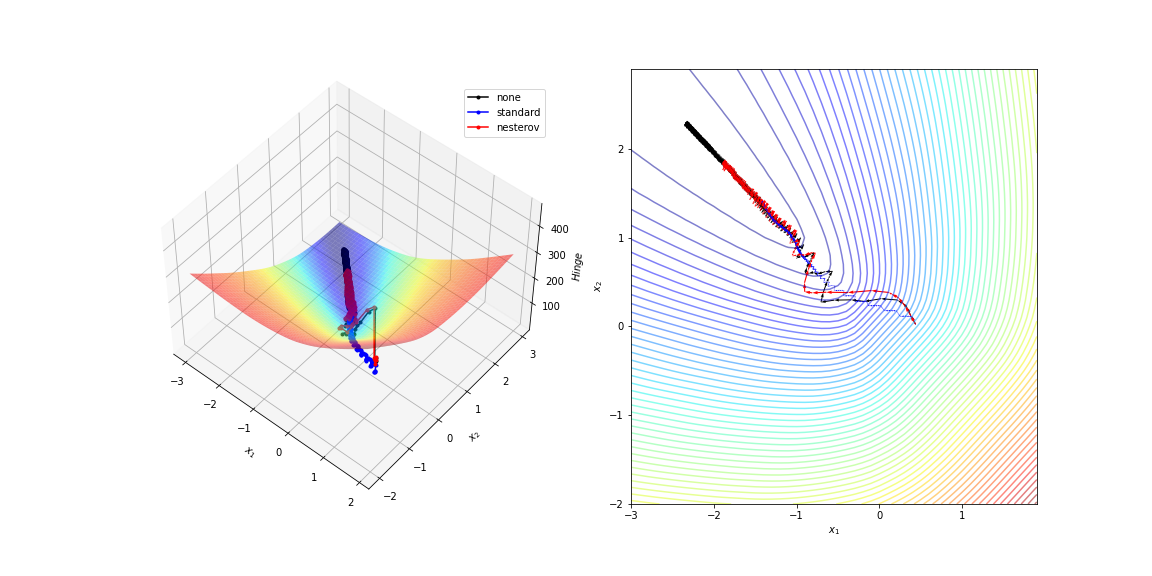
\includegraphics[scale=0.5]{img/svc_hinge_loss.png}
  	\caption{SVC Hinge loss}
  	\label{fig:svc_hinge_loss}
\end{figure}

\subsubsection{Squared Hinge loss}

Since smoothed versions of objective functions may be preferred for optimization, we can reformulate \ref{eq:svc_hinge} as:

\begin{equation} \label{eq:svc_sq_hinge}
    \min_{w,b} \frac{1}{2} \Vert w \Vert^2 + C \sum_{i=1}^n \max(0, 1 - y_i (w^T x_i + b))^2
\end{equation}

where we make use of the \emph{squared hinge} loss that quadratically penalized slacks $\xi$ and is called $\mathcal{L}_2$-SVC.

\begin{figure}[h!]
	\centering
  	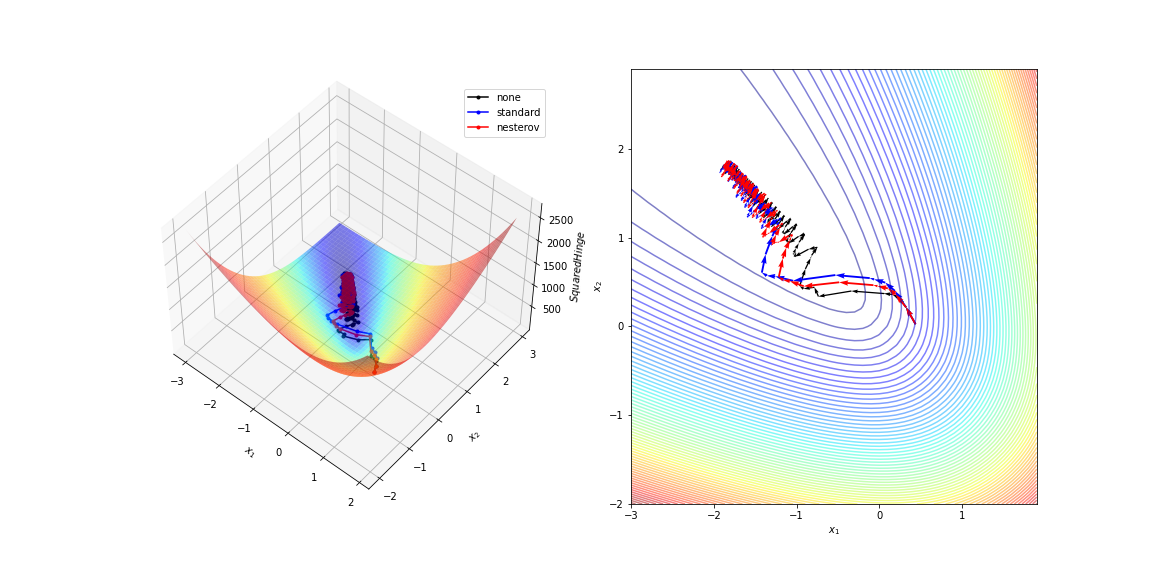
\includegraphics[scale=0.5]{img/svc_squared_hinge_loss.png}
  	\caption{SVC Squared Hinge loss}
  	\label{fig:svc_squared_hinge_loss}
\end{figure}

\bigskip
\bigskip

To simplify the notation and so also the design of the algorithms, the simplest approach to learn the bias term $b$ is that of including that into the \emph{regularization term}; so we can rewrite \ref{eq:svc_hinge} and \ref{eq:svc_sq_hinge} as follows:

\begin{equation} \label{eq:primal_svc_hinge1}
    \min_{w,b} \frac{1}{2} (\Vert w \Vert^2 + b^2) + C \sum_{i=1}^n \mathcal{L}(w;x_i,y_i)
\end{equation}

or, equivalently, by augmenting the weight vector $w$ with the bias term $b$ and each instance $x_i$ with an additional dimension, i.e., with constant value equal to 1:

\begin{equation} \label{eq:primal_svc_hinge2}
    \begin{aligned}
        \min_{w} \quad & \frac{1}{2} \Vert \bar{w} \Vert^2 + C \sum_{i=1}^n \mathcal{L}(w;\bar{x}_i,y_i) \\
            \textrm{where} \quad & \bar{w}^T = [w^T, b] \\ & \bar{x}_i^T = [x_i^T, 1]
    \end{aligned}
\end{equation}

with the advantages of having convex properties of the objective function useful for convergence analysis and the possibility to directly apply algorithms designed for models without the bias term.

Notice that in terms of numerical optimization the formulations \ref{eq:svc_hinge} and \ref{eq:svc_sq_hinge} are not equivalent to \ref{eq:primal_svc_hinge1} or \ref{eq:primal_svc_hinge2} since in the first one the bias term $b$ does not contribute to the \emph{regularization term}, so the SVM formulation is based on an unregularized bias term $b$, as highlighted by the \emph{statistical learning theory}. But, in machine learning sense, numerical experiments in \cite{hsu2002simple} show that the accuracy does not vary much when the bias term $b$ is embedded into the weight vector $w$.

\subsection{Dual Formulations}

\subsubsection{Wolfe Dual}

To reformulate the \ref{eq:quad_svc_obj} as a \emph{Wolfe dual}, we need to allocate the Lagrange multipliers $\alpha_i\geq 0, \mu_i \geq 0 \ \forall_i$:

\begin{equation} \label{eq:svc_wolfe_dual}
    \max_{\alpha,\mu} \min_{w,b,\xi} \mathcal{W}(w,b,\xi,\alpha,\mu) = \frac{1}{2}\Vert w\Vert^{2}+C\sum_{i=1}^n\xi_i-\sum_{i=1}^n\alpha_i(y_i(w^T x_i + b)-1+\xi_i)-\sum_{i=1}^n\mu_i\xi_i
\end{equation}

We wish to find the $w$, $b$ and $\xi_i$ which minimizes, and the $\alpha$ and $\mu$ which maximizes $\mathcal{W}$, provided $\alpha_i\geq 0, \mu_i \geq 0 \ \forall_i$. We can do this by differentiating $\mathcal{W}$ wrt $w$ and $b$ and setting the derivatives to 0:

\begin{equation} \label{eq:svc_wolfe_der_w}
	\frac{\partial \mathcal{W}}{\partial w}=w-\sum_{i=1}^{n}\alpha_i y_i x_i \Rightarrow w=\sum_{i=1}^{n}\alpha_i y_i x_i
\end{equation}

\begin{equation} \label{eq:svc_wolfe_der_b}
	\frac{\partial \mathcal{W}}{\partial b}=-\sum_{i=1}^{n}\alpha_i y_i\Rightarrow\sum_{i=1}^{n}\alpha_i y_i=0
\end{equation}

\begin{equation} \label{eq:svc_wolfe_der_xi}
	\frac{\partial \mathcal{W}}{\partial\xi_i}=0\Rightarrow C=\alpha_i+\mu_i
\end{equation}

Substituting \ref{eq:svc_wolfe_der_w} and \ref{eq:svc_wolfe_der_b} into \ref{eq:svc_wolfe_dual} together with $\mu_i\geq 0 \ \forall_i$, which implies that $\alpha\leq C$, gives a new formulation being dependent on $\alpha$. We therefore need to find:

\begin{equation} \label{eq:svc_max_wolfe_dual}
	\begin{aligned}
    	\max_{\alpha} \mathcal{W}(\alpha) &= \sum_{i=1}^{n}\alpha_i - \frac{1}{2}\sum_{i,j}\alpha_i\alpha_j y_i y_j \langle x_i, x_j \rangle \\
    	&= \sum_{i=1}^{n}\alpha_i - \frac{1}{2}\sum_{i,j}\alpha_i Q_{ij}\alpha_j \ \text{where} \ Q_{ij} = y_i y_j \langle x_i, x_j \rangle \\
    	&= \sum_{i=1}^{n}\alpha_i - \frac{1}{2}\alpha^T Q\alpha \ \text{subject to} \ 0\leq\alpha_i\leq C \ \forall_i, \sum_{i=1}^{n}\alpha_i y_i=0 
	\end{aligned}
\end{equation}

or, equivalently:

\begin{equation} \label{eq:svc_min_wolfe_dual}
    \begin{aligned}
        \min_{\alpha} \quad & \frac{1}{2}\alpha^T Q\alpha+q^T\alpha \\
            \textrm{subject to} \quad & 0\leq\alpha_i\leq C \ \forall_i \\ & y^T\alpha=0
    \end{aligned}
\end{equation}

where $q^T = [1, \dots, 1]$.

By solving \ref{eq:svc_min_wolfe_dual} we will know $\alpha$ and, from \ref{eq:svc_wolfe_der_w}, we will get $w$, so we need to calculate $b.$

We know that any data point satisfying \ref{eq:svc_wolfe_der_b} which is a support vector $x_s$ will have the form:

\begin{equation} \label{eq:svc_sv_const1}
	y_s(w^T x_s + b)=1
\end{equation}

and, by substituting in \ref{eq:svc_wolfe_der_w}, we get:

\begin{equation} \label{eq:svc_sv_const2}
	y_s\big(\sum_{m\in S}\alpha_m y_m \langle x_m, x_s \rangle +b\big)=1
\end{equation}

where $s$ denotes the set of indices of the support vectors and is determined by finding the indices $i$ where $\alpha_i>0$, i.e., nonzero Lagrange multipliers.

Multiplying through by $y_s$ and then using $y_s^2=1$ from \ref{eq:svc_consts}:

\begin{equation} \label{eq:svc_sv_sq_const2}
	y_s^2\big(\sum_{m\in S}\alpha_m y_m \langle x_m, x_s \rangle +b\big)=y_s
\end{equation}

\begin{equation} \label{eq:svc_b}
	b=y_s-\sum_{m\in S}\alpha_m y_m \langle x_m, x_s \rangle
\end{equation}

Instead of using an arbitrary support vector $x_s$, it is better to take an average over all of the support vectors in $S$:

\begin{equation} \label{eq:svc_b_avg}
	b=\frac{1}{N_s}\sum_{s\in S} y_s-\sum_{m\in S}\alpha_m y_m \langle x_m, x_s \rangle
\end{equation}

We now have the variables $w$ and $b$ that define our separating hyperplane's optimal orientation and hence our support vector machine. Each new point $x'$ is classified by evaluating:

\begin{equation} \label{eq:svc_pred}
    y'=\operatorname{sgn}\big(\sum_{i=1}^{n}\alpha_i y_i\langle x_i, x' \rangle+b\big)
\end{equation}

From \ref{eq:svc_min_wolfe_dual} we can notice that the equality constraint $y^T \alpha = 0$ arises form the stationarity condition $\partial_{{b}} \mathcal{W}=0$. So, again, for simplicity, we can again consider the bias term $b$ embedded into the weight vector. We report below the box-constrained dual formulation \cite{hsu2002simple} that arises from the primal \ref{eq:primal_svc_hinge1, eq:primal_svc_hinge2} where the bias term $b$ is embedded into the weight vector $w$:

\begin{equation} \label{eq:svc_min_bcqp_wolf_dual}
    \begin{aligned}
        \min_{\alpha} \quad & \frac{1}{2} \alpha^T (Q + yy^T)\alpha+q^T\alpha \\
            \textrm{subject to} \quad & 0\leq\alpha_i\leq C \ \forall_i
    \end{aligned}
\end{equation}

\subsubsection{Lagrangian Dual}

In order to relax the constraints in the \emph{Wolfe dual} formulation \ref{eq:svc_min_wolfe_dual} we define the problem as a \emph{Lagrangian dual} relaxation by embedding them into objective function, so we need to allocate the Lagrangian multipliers $\mu \geq 0, \lambda_+ \geq 0$, $\lambda_- \geq 0$:

\begin{equation} \label{eq:svc_lagrangian_dual}
	\begin{aligned}
		    \max_{\mu,\lambda_+,\lambda_-} \min_{\alpha} \mathcal{L}(\alpha,\mu,\lambda_+,\lambda_-) &= \frac{1}{2} \alpha^T Q\alpha+q^T\alpha - \mu^T (y^T \alpha) - \lambda_+^T (u - \alpha) - \lambda_-^T \alpha \\
    &= \frac{1}{2} \alpha^T Q\alpha + (q - \mu y + \lambda_+ - \lambda_-)^T \alpha - \lambda_+^T u
	\end{aligned}
\end{equation}

where the upper bound $u^T = [C, \dots, C]$.

Taking the derivative of the Lagrangian $\mathcal{L}$ wrt $\alpha$ and settings it to 0 gives:

\begin{equation} \label{eq:svc_lagrangian_der_a}
	\frac{\partial \mathcal{L}}{\partial \alpha}=0\Rightarrow Q \alpha + (q - \mu y + \lambda_+ - \lambda_-) = 0
\end{equation}

With $\alpha$ optimal solution of the linear system:

\begin{equation} \label{eq:svc_lagrangian_sol}
    Q \alpha = - (q - \mu y + \lambda_+ - \lambda_-)
\end{equation}

the gradient wrt $\mu$, $\lambda_+$ and $\lambda_-$ are:

\begin{equation} \label{eq:svc_lagrangian_der_mu}
	\frac{\partial \mathcal{L}}{\partial \mu}=-y \alpha
\end{equation}

\begin{equation} \label{eq:svc_lagrangian_der_lp}
	\frac{\partial \mathcal{L}}{\partial \lambda_+}=\alpha - u
\end{equation}

\begin{equation} \label{eq:svc_lagrangian_der_lm}
    \frac{\partial \mathcal{L}}{\partial \lambda_-}=-\alpha
\end{equation}

If the Hessian matrix Q is indefinite, i.e., the Lagrangian function is not strictly convex since it will be linear along the eigenvectors correspondent to the null eigenvalues, the Lagrangian dual relaxation will be nondifferentiable, so it will have infinite solutions and for each of them it will have a different subgradient. In order to compute the gradient, we will choose $\alpha$ in such a way as the one that minimizes the residue, i.e. the least-squares solution:

\begin{equation} \label{eq:svc_lagrangian_krylov_sol}
	\begin{aligned}
			\min_{\alpha \in K_n(Q, b)} \quad & \Vert Q \alpha - b \Vert \\ 
			\textrm{where} \quad & b = - (q - \mu y + \lambda_+ - \lambda_-)
	\end{aligned}
\end{equation}

Since we are dealing with a symmetric but indefinite linear system we will choose a well-known Krylov method that performs the Lanczos iterate, i.e., symmetric Arnoldi iterate, called \emph{minres}, i.e., symmetric \emph{gmres}, which computes the vector $\alpha$ that minimizes $\Vert Q \alpha - b \Vert$ among all vectors in $K_n(Q, b) = span(b, Qb, Q^2b, \dots, Q^{n-1}b)$.

\bigskip
\bigskip

From \ref{eq:svc_min_wolfe_dual} we can notice that the equality constraint $y^T \alpha = 0$ arises form the stationarity condition $\partial_{{b}} \mathcal{W}=0$. So, again, for simplicity, we can again consider the bias term $b$ embedded into the weight vector. In this way the dimensionality of \ref{eq:eq:svc_lagrangian_dua} is reduced of 1/3 by removing the multipliers $\mu$ which was allocated to control the equality constraint $y^T \alpha=0$, so we will end up solving exactly the problem \ref{eq:svc_min_bcqp_wolf_dual}.

\begin{equation} \label{eq:svc_bcqp_lagrangian_dual}
	\begin{aligned}
    	\max_{\lambda_+,\lambda_-} \min_{\alpha} \mathcal{L}(\alpha,\lambda_+,\lambda_-) &= \frac{1}{2} \alpha^T (Q + yy^T)\alpha+q^T\alpha - \lambda_+^T (u - \alpha) - \lambda_-^T \alpha \\
    &= \frac{1}{2} \alpha^T (Q + yy^T)\alpha + (q + \lambda_+ - \lambda_-)^T \alpha - \lambda_+^T u
	\end{aligned}
\end{equation}

where, again, the upper bound $u^T = [C, \dots, C]$.

Now, taking the derivative of the Lagrangian $\mathcal{L}$ wrt $\alpha$ and settings it to 0 gives:

\begin{equation} \label{eq:svc_bcqp_lagrangian_der_a}
	\frac{\partial \mathcal{L}}{\partial \alpha}=0\Rightarrow (Q + yy^T) \alpha + (q + \lambda_+ - \lambda_-) = 0
\end{equation}

With $\alpha$ optimal solution of the linear system:

\begin{equation} \label{eq:svc_bcqp_lagrangian_sol}
    (Q + yy^T) \alpha = - (q + \lambda_+ - \lambda_-)
\end{equation}

the gradient wrt $\lambda_+$ and $\lambda_-$ are:

\begin{equation} \label{eq:svc_bcqp_lagrangian_der_lp}
	\frac{\partial \mathcal{L}}{\partial \lambda_+}=\alpha - u
\end{equation}

\begin{equation} \label{eq:svc_bcqp_lagrangian_der_lm}
    \frac{\partial \mathcal{L}}{\partial \lambda_-}=-\alpha
\end{equation}


\pagebreak

\section{Linear Support Vector Regression}

In the case of regression the goal is to predict a real-valued output for $y'$ so that our training data is of the form:

\begin{equation}
	\{(x_i,y_i), x\in\Re^m, y_i\in\Re, i=1, \dots, n\} \label{eq:svr_data}
\end{equation}

The regression SVM use a loss function that not allocating a penalty if the predicted value $y'_i$ is less than a distance $\epsilon$ away from the actual value $y_i$, i.e., if $|y_i-y'_i| \leq \epsilon$, where $y'_i = w^T x_i + b$. The region bound by $y'_i\pm\epsilon \ \forall_i$ is called an $\epsilon$-insensitive tube. The output variables which are outside the tube are given one of two slack variable penalties depending on whether they lie above, $\xi^+$, or below, $\xi^-$, the tube, provided $\xi^+ \geq 0$ and $\xi^- \geq 0 \ \forall_i$:

\begin{equation} \label{eq:svr_consts}
	\begin{aligned}
		& y_i\leq y'_i+\epsilon+\xi^+ \ \forall_i \\
    	& y_i\geq y'_i-\epsilon-\xi^- \ \forall_i \\
    	& \xi_i^+, \xi_i^- \geq 0 \ \forall_i
	\end{aligned}
\end{equation}

The objective function for SVR can then be written as:

\begin{equation} \label{eq:quad_svr_obj}
    \begin{aligned}
        \min_{w,b,\xi^+,\xi^-} \quad & \frac{1}{2} \| w \|^2 + C \sum_{i=1}^n (\xi_i^+ + \xi_i^-) \\
            \text{subject to} \quad & y_i - w^T x_i - b \leq \epsilon + \xi_i^+ \ \forall_i \\ & w^T x_i + b - y_i \leq \epsilon + \xi_i^- \ \forall_i \\ & \xi_i^+, \xi_i^- \geq 0 \ \forall_i
    \end{aligned}
\end{equation}

\begin{figure}[h!]
	\centering
  	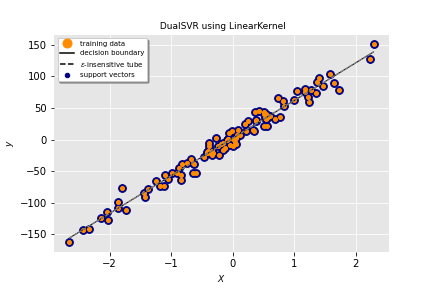
\includegraphics[scale=0.6]{img/linear_dual_svr_hyperplane.png}
  	\caption{Linear SVR hyperplane}
  	\label{fig:linear_dual_svr_hyperplane}
\end{figure}

\subsection{Epsilon-insensitive loss}

The \emph{epsilon-insensitive} loss is defined as:

\begin{equation} \label{eq:eps_loss1}
	\mathcal{L}_\epsilon = 
	\begin{cases}
		0 & \text{if} \ |y - (w^T x + b)| \leq \epsilon \\
		|y - (w^T x + b)| - \epsilon & \text{otherwise} \\
	\end{cases}
\end{equation}

or, equivalently:

\begin{equation} \label{eq:eps_loss2}
	\mathcal{L}_\epsilon = \max(0, |y - (w^T x + b)| - \epsilon)
\end{equation}

As the \emph{hinge} loss, also the \emph{epsilon-insensitive} loss is a nondifferentiable convex function due to its nonsmoothness in $\pm\epsilon$, but has a subgradient wrt $w$ that is given by:

\begin{equation} \label{eq:eps_loss_der}
	\frac{\partial \mathcal{L_\epsilon}}{\partial w}=
		\begin{cases}
            (y - (w^T x + b)) x & \text{if} \ |y - (w^T x + b)| > \epsilon \\
            0 & \text{otherwise} \\ 
        \end{cases}
\end{equation}

\subsubsection{Primal formulation}

The general primal unconstrained formulation takes the same form of \ref{eq:primal_svc}.

The quadratic optimization problem \ref{eq:quad_svr_obj} can be equivalently formulated as: 

\begin{equation} \label{eq:svr_eps}
	\min_{w,b} \frac{1}{2} \| w \|^2 + C \sum_{i=1}^n \max(0, |y_i - (w^T x_i + b)| - \epsilon)
\end{equation}

where we make use of the \emph{epsilon-insensitive} loss \ref{eq:eps_loss1} or \ref{eq:eps_loss2}.

The above formulation penalizes slacks $\xi$ linearly and is called $\mathcal{L}_1$-SVR.

\begin{figure}[h!]
	\centering
  	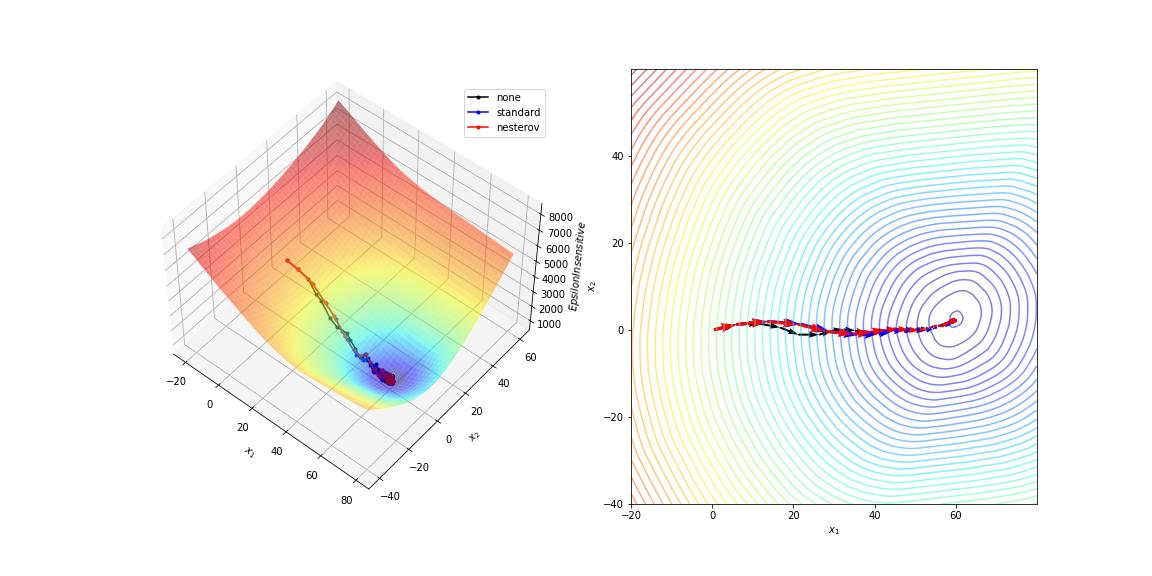
\includegraphics[scale=0.4]{img/svr_eps_loss.png}
  	\caption{SVR Epsilon-insensitive loss with different optimization steps}
  	\label{fig:svr_eps_loss}
\end{figure}

\subsubsection{Wolfe Dual formulation}

To reformulate the \ref{eq:quad_svr_obj} as a \emph{Wolfe dual}, we introduce the Lagrange multipliers $\alpha_i^+ \geq 0, \alpha_i^- \geq 0, \mu_i^+ \geq 0, \mu_i^- \geq 0 \ \forall_i$:

\begin{equation} \label{eq:svr_wolfe_dual}
	\begin{aligned}
    	\max_{\alpha^+,\alpha^-,\mu^+,\mu^-} \min_{w,b,\xi^+,\xi^-} \mathcal{W}(w,b,\xi^+,\xi^-,\alpha^+,\alpha^-,\mu^+,\mu^-) = \frac{1}{2} \| w \|^2 + C \sum_{i=1}^n (\xi_i^+ + \xi_i^-)-\sum_{i=1}^n (\mu_i^+ \xi_i^+ + \mu_i^- \xi_i^-) \\ -\sum_{i=1}^n \alpha_i^+(\epsilon+\xi_i^+ + y'_i-y_i)-\sum_{i=1}^n \alpha_i^-(\epsilon+\xi_i^- - y'_i+y_i)
	\end{aligned}
\end{equation}

Substituting for $y_i$, differentiating wrt $w, b, \xi^+$, $\xi^-$ and setting the derivatives to $0$ gives:

\begin{equation} \label{eq:svr_wolfe_der_w}
	\frac{\partial \mathcal{W}}{\partial w}=w-\sum_{i=1}^n (\alpha_i^+ - \alpha_i^-) x_i \Rightarrow w=\sum_{i=1}^n (\alpha_i^+ - \alpha_i^-) x_i
\end{equation}

\begin{equation} \label{eq:svr_wolfe_der_b}
	\frac{\partial \mathcal{W}}{\partial b}=-\sum_{i=1}^n (\alpha_i^+ - \alpha_i^-)\Rightarrow \sum_{i=1}^n (\alpha_i^+ - \alpha_i^-)=0
\end{equation}

\begin{equation}\label{eq:svr_wolfe_der_xip}
	\frac{\partial \mathcal{W}}{\partial\xi_i^+}=0\Rightarrow C=\alpha_i^+ + \mu_i^+
\end{equation}

\begin{equation} \label{eq:svr_wolfe_der_xim}
	\frac{\partial \mathcal{W}}{\partial\xi_i^-}=0\Rightarrow C=\alpha_i^- + \mu_i^-
\end{equation}

Substituting \ref{eq:svr_wolfe_der_w} and \ref{eq:svr_wolfe_der_b} in, we now need to maximize $\mathcal{W}$ wrt $\alpha_i^+$ and $\alpha_i^-$, where $\alpha_i^+ \geq 0,\ \alpha_i^- \geq 0 \ \forall_i$:

\begin{equation} \label{eq:svr_max_wolfe_dual}
    \max_{\alpha^+,\alpha^-} \mathcal{W}(\alpha^+,\alpha^-) = \sum_{i=1}^n y_i(\alpha_i^+ - \alpha_i^-)-\epsilon\sum_{i=1}^n (\alpha_i^+ + \alpha_i^-)-\frac{1}{2}\sum_{i,j}(\alpha_i^+ - \alpha_i^-)\langle x_i, x_j \rangle(\alpha_j ^+ - \alpha_j ^-)
\end{equation}

Using $\mu_i^+ \geq 0$ and $\mu_i^- \geq 0$ together with \ref{eq:svr_wolfe_der_w} and \ref{eq:svr_wolfe_der_b} means that $\alpha_i^+ \leq C$ and $\alpha_i^- \leq C$. We therefore need to find:

\begin{equation} \label{eq:svr_min_wolfe_dual}
    \begin{aligned}
        \min_{\alpha^+,\alpha^-} \quad & \frac{1}{2}(\alpha^+ - \alpha^-)^TK(\alpha^+ - \alpha^-)+\epsilon q^T(\alpha^+ + \alpha^-)-y^T(\alpha^+ - \alpha^-) \\
            \text{subject to} \quad & 0\leq\alpha_i^+,\alpha_i^- \leq C \ \forall_i \\ & q^T(\alpha^+ - \alpha^-)=0
    \end{aligned}
\end{equation}

where $q^T = [1, \dots, 1]$.

We can write the \ref{eq:svr_min_wolfe_dual} in a standard quadratic form as:

\begin{equation}
    \begin{aligned} \label{eq:svr_min_qp_wolfe_dual}
        \min_{\alpha} \quad & \frac{1}{2}\alpha^T Q\alpha-q^T\alpha \\
            \text{subject to} \quad & 0\leq\alpha_i\leq C \ \forall_i \\ & e^T\alpha=0
    \end{aligned}
\end{equation}

where the Hessian matrix $Q$ is 
$
\begin{bmatrix}
K & -K\\
-K & K 
\end{bmatrix}$
, $q$ is 
$
\begin{bmatrix}
-y\\
y
\end{bmatrix}$ + $\epsilon$
, and $e$ is 
$
\begin{bmatrix}
1\\
-1
\end{bmatrix}$.

Each new predictions $y'$ can be found using:

\begin{equation} \label{eq:svr_pred}
    y'= \sum_{i=1}^n (\alpha_i^+ - \alpha_i^-)\langle x_i, x' \rangle+b
\end{equation}

A set $S$ of support vectors $x_s$ can be created by finding the indices $i$ where $0\leq\alpha\leq C$ and $\xi_i^+=0$ or $\xi_i^-=0$.

This gives us:

\begin{equation} \label{eq:svr_b}
    b=y_s-\epsilon-\sum_{m\in S}(\alpha_m^+ -\alpha_m^-) \langle x_m, x_s \rangle
\end{equation}

As before it is better to average over all the indices $i$ in $S$:

\begin{equation} \label{eq:svr_b_avg}
    b=\frac{1}{N_s}\sum_{s\in S}y_s-\epsilon-\sum_{m \in S}(\alpha_m^+ - \alpha_m^-)\langle x_m, x_s \rangle
\end{equation}

From \ref{eq:svr_min_qp_wolfe_dual} we can notice that the equality constraint $e^T \alpha = 0$ arises form the stationarity condition $\partial_{{b}} \mathcal{W}=0$. So, again, for simplicity, we can again consider the bias term $b$ embedded into the weight vector. We report below the box-constrained dual formulation \cite{hsu2002simple} that arises from the primal \ref{eq:primal_svc_hinge1} or \ref{eq:primal_svc_hinge2} where the bias term $b$ is embedded into the weight vector $w$:

\begin{equation} \label{eq:svr_min_bcqp_wolf_dual}
    \begin{aligned}
        \min_{\alpha} \quad & \frac{1}{2} \alpha^T (Q + ee^T)\alpha+q^T\alpha \\
            \text{subject to} \quad & 0\leq\alpha_i\leq C \ \forall_i
    \end{aligned}
\end{equation}

\subsubsection{Lagrangian Dual formulation}

In order to relax the constraints in the \emph{Wolfe dual} formulation \ref{eq:svr_min_wolfe_dual} we define the problem as a \emph{Lagrangian dual} relaxation by embedding them into objective function, so we need to allocate the Lagrangian multipliers $\mu \geq 0, \lambda_+ \geq 0$, $\lambda_- \geq 0$:

\begin{equation} \label{eq:svr_lagrangian_dual}
	\begin{aligned}
		    \max_{\mu,\lambda_+,\lambda_-} \min_{\alpha} \mathcal{L}(\alpha,\mu,\lambda_+,\lambda_-) &= \frac{1}{2} \alpha^T Q\alpha+q^T\alpha - \mu^T (e^T \alpha) - \lambda_+^T (u - \alpha) - \lambda_-^T \alpha \\
    &= \frac{1}{2} \alpha^T Q\alpha + (q - \mu e + \lambda_+ - \lambda_-)^T \alpha - \lambda_+^T u
	\end{aligned}
\end{equation}

where the upper bound $u^T = [C, \dots, C]$.

Taking the derivative of the Lagrangian $\mathcal{L}$ wrt $\alpha$ and settings it to 0 gives:

\begin{equation} \label{eq:svr_lagrangian_der_a}
	\frac{\partial \mathcal{L}}{\partial \alpha}=0\Rightarrow Q \alpha + (q - \mu e + \lambda_+ - \lambda_-) = 0
\end{equation}

With $\alpha$ optimal solution of the linear system:

\begin{equation} \label{eq:svr_lagrangian_sol}
    Q \alpha = - (q - \mu e + \lambda_+ - \lambda_-)
\end{equation}

the gradient wrt $\mu$, $\lambda_+$ and $\lambda_-$ are:

\begin{equation} \label{eq:svr_lagrangian_der_mu}
	\frac{\partial \mathcal{L}}{\partial \mu}=-e \alpha
\end{equation}

\begin{equation} \label{eq:svr_lagrangian_der_lp}
	\frac{\partial \mathcal{L}}{\partial \lambda_+}=\alpha - u
\end{equation}

\begin{equation} \label{eq:svr_lagrangian_der_lm}
    \frac{\partial \mathcal{L}}{\partial \lambda_-}=-\alpha
\end{equation}

If the Hessian matrix Q is not positive definite, i.e., the Lagrangian function is not strictly convex since it will be linear along the eigenvectors correspondent to the null eigenvalues and so it will be unbounded below, the Lagrangian dual relaxation will be nondifferentiable, so it will have infinite solutions and for each of them it will have a different subgradient. In order to compute an approximation of the gradient, we will choose $\alpha$ in such a way as the one that minimizes the norm of the residual:

\begin{equation} \label{eq:svr_lagrangian_krylov_sol}
	\begin{aligned}
		\min_{\alpha_n \in K_n(Q, b)} \quad & \| Q \alpha_n - b \| \\ 
		\text{where} \quad & b = - (q - \mu e + \lambda_+ - \lambda_-)
	\end{aligned}
\end{equation}

Since we are dealing with a symmetric but indefinite linear system we will choose a well-known Krylov method that performs the Lanczos iterate, i.e., symmetric Arnoldi iterate, called \emph{minres}, i.e., symmetric \emph{gmres}, to compute the vector $\alpha_n$ that minimizes the norm of the residual $r_n = Q \alpha_n - b$ among all vectors in $K_n(Q, b) = span(b, Qb, Q^2b, \dots, Q^{n-1}b)$.

\bigskip

From \ref{eq:svr_min_qp_wolfe_dual} we can notice that the equality constraint $e^T \alpha = 0$ arises form the stationarity condition $\partial_{{b}} \mathcal{W}=0$. So, again, for simplicity, we can again consider the bias term $b$ embedded into the weight vector. In this way the dimensionality of \ref{eq:svr_lagrangian_dual} is reduced of 1/3 by removing the multipliers $\mu$ which was allocated to control the equality constraint $e^T \alpha=0$, so we will end up solving exactly the problem \ref{eq:svr_min_bcqp_wolf_dual}.

\begin{equation} \label{eq:svr_bcqp_lagrangian_dual}
	\begin{aligned}
    	\max_{\lambda_+,\lambda_-} \min_{\alpha} \mathcal{L}(\alpha,\lambda_+,\lambda_-) &= \frac{1}{2} \alpha^T (Q + ee^T)\alpha+q^T\alpha - \lambda_+^T (u - \alpha) - \lambda_-^T \alpha \\
    &= \frac{1}{2} \alpha^T (Q + ee^T)\alpha + (q + \lambda_+ - \lambda_-)^T \alpha - \lambda_+^T u
	\end{aligned}
\end{equation}

where, again, the upper bound $u^T = [C, \dots, C]$.

Now, taking the derivative of the Lagrangian $\mathcal{L}$ wrt $\alpha$ and settings it to 0 gives:

\begin{equation} \label{eq:svr_bcqp_lagrangian_der_a}
	\frac{\partial \mathcal{L}}{\partial \alpha}=0\Rightarrow (Q + ee^T) \alpha + (q + \lambda_+ - \lambda_-) = 0
\end{equation}

With $\alpha$ optimal solution of the linear system:

\begin{equation} \label{eq:svr_bcqp_lagrangian_sol}
    (Q + ee^T) \alpha = - (q + \lambda_+ - \lambda_-)
\end{equation}

the gradient wrt $\lambda_+$ and $\lambda_-$ are:

\begin{equation} \label{eq:svr_bcqp_lagrangian_der_lp}
	\frac{\partial \mathcal{L}}{\partial \lambda_+}=\alpha - u
\end{equation}

\begin{equation} \label{eq:svr_bcqp_lagrangian_der_lm}
    \frac{\partial \mathcal{L}}{\partial \lambda_-}=-\alpha
\end{equation}

\subsection{Squared Epsilon-insensitive loss}

The \emph{squared epsilon-insensitive} loss is defined as:

\begin{equation} \label{eq:squared_eps_loss1}
	\mathcal{L}_\epsilon^2 = 
	\begin{cases}
		0 & \text{if} \ |y - (w^T x + b)| \leq \epsilon \\
		(|y - (w^T x + b)| - \epsilon)^2 & \text{otherwise} \\
	\end{cases}
\end{equation}

or, equivalently:

\begin{equation} \label{eq:squared_eps_loss2}
	\mathcal{L}_\epsilon^2 = \max(0, |y - (w^T x + b)| - \epsilon)^2
\end{equation}

As the \emph{squared hinge} loss, also the \emph{squared epsilon-insensitive} loss is a strictly convex function and it has a gradient wrt $w$ that is given by:

\begin{equation} \label{eq:squared_eps_loss_der}
	\frac{\partial \mathcal{L}_\epsilon^2}{\partial w}=
		\begin{cases}
            2 ((y - (w^T x + b)) x) & \text{if} \ |y - (w^T x + b)| > \epsilon \\
            0 & \text{otherwise} \\ 
        \end{cases}
\end{equation}

\subsubsection{Primal formulation}

To provide a continuously differentiable function the optimization problem \ref{eq:svr_eps} can be formulated as: 

\begin{equation} \label{eq:svr_squared_eps}
    \min_{w,b} \frac{1}{2} \| w \|^2 + C \sum_{i=1}^n \max(0, |y_i - (w^T x_i + b)| - \epsilon)^2
\end{equation}

where we make use of the \emph{squared epsilon-insensitive} loss that quadratically penalized slacks $\xi$ and is called $\mathcal{L}_2$-SVR.

\begin{figure}[h!]
	\centering
  	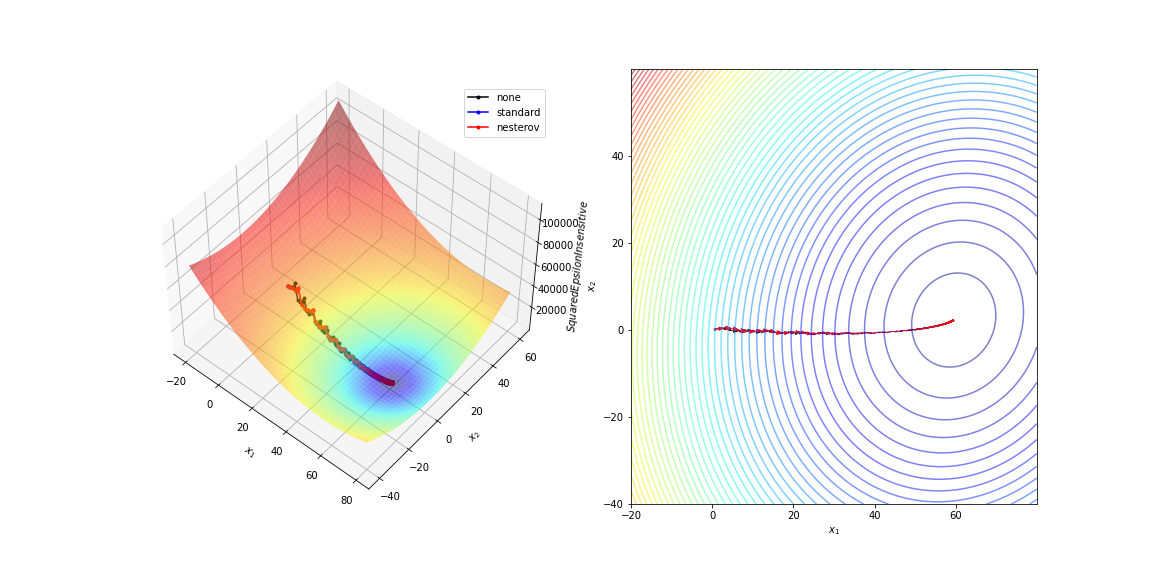
\includegraphics[scale=0.4]{img/svr_squared_eps_loss.png}
  	\caption{SVC Squared Epsilon-insensitive loss with different optimization steps}
  	\label{fig:svr_squared_eps_loss}
\end{figure}


\pagebreak

\section{Nonliner Support Vector Machines}

When applying our SVM to linearly separable data we have started by creating a matrix $Q$ from the dot product of our input variables:

\begin{equation}
	Q_{ij}=y_i y_j k(x_i,x_j) \tag{3.1}
\end{equation}

where $k(x_i,x_j)$ is an example of a family of functions called \emph{kernel functions} and:  

\begin{equation}
	k(x_i,x_j)=\langle x_i, x_j \rangle= x_i^T x_j \tag{3.2}
\end{equation}

is known as \emph{linear} kernel.

The reason that this \emph{kernel trick} is useful is that there are many classification/regression problems that are not linearly separable/regressable in the space of the inputs $x$, which might be in a higher dimensionality feature space given a suitable mapping $x \rightarrow \phi(x)$.

\subsection{Polynomial kernel}

The \emph{polynomial} kernel is defined as:

\begin{equation}
	k(x_i,x_j)=(\gamma \langle x_i, x_j\rangle + r)^d \tag{3.3}
\end{equation}

where $\gamma$ define how far the influence of a single training example reaches (low values meaning ‘far’ and high values meaning ‘close’).

\subsection{Gaussian kernel}

The \emph{gaussian} kernel is defined as:

\begin{equation}
	k(x_i,x_j)=\exp(-\frac{\|x_i-x_j\|^2}{2\sigma^2}) \tag{3.4a}
\end{equation}

or, equivalently, as:

\begin{equation}
	k(x_i,x_j)=\exp(-\gamma \|x_i-x_j\|^2) \tag{3.4b}
\end{equation}

where $\displaystyle \gamma=\frac{1}{2\sigma^2}$ define how far the influence of a single training example reaches (low values meaning ‘far’ and high values meaning ‘close’).

\pagebreak

\section{Optimization}

In order to explain the \emph{convergence} and \emph{efficiency} properties of the following numerical and optimization methods, we need to introduce some preliminary definitions about \emph{convexity} and the \emph{L-smoothness} of a function.

First of all, we give three different but equivalent definitions of convexity in terms of the function itself, the Jacobian and the Hessian.

\begin{definition}[Convexity]
We say that a function $\mathcal{L}: \Re^m \rightarrow \Re$ is convex if: 
$$ 
\mathcal{L}(\lambda x + (1 - \lambda) y ) \leq \lambda \mathcal{L}(x) + (1 - \lambda) \mathcal{L}(y) \ \forall \ x, y \in \Re^m, \lambda \in [0,1] 
$$
\end{definition}

\begin{definition}[Convexity - Jacobian]
We say that a differentiable function $\mathcal{L}: \Re^m \rightarrow \Re$ is convex iff: 
$$
\mathcal{L}(x) \geq \mathcal{L}(y) + \langle \nabla \mathcal{L}(y), x - y \rangle \ \forall \ x, y \in \Re^m
$$
\end{definition}

\begin{definition}[Convexity - Hessian]
We say that a twice differentiable function, i.e., the Hessian matrix is \emph{symmetric}, $\mathcal{L}: \Re^m \rightarrow \Re$ is convex iff: 
$$
\nabla^2 \mathcal{L}(x) \succeq 0 \ \forall \ x \in \Re^m
$$
i.e., the Hessian matix is \emph{positive semidefinite}.
\end{definition}

The definitions of \emph{strong convexity} and \emph{L-smoothness} below will be useful.

\begin{definition}[Strong Convexity]
We say that a function $\mathcal{L}: \Re^m \rightarrow \Re$ is $\mu$-strongly convex if:
$$
\mathcal{G}(x) = \mathcal{L}(x) - \frac{\mu}{2} \| x \|^2
$$
is convex. The latter, in terms of the Jacobian, is equivalent to:
$$
\mathcal{L}(x) \geq \mathcal{L}(y) + \langle \nabla \mathcal{L}(y), x - y \rangle + \frac{\mu}{2} \| x - y \|^2 \ \forall \ x, y \in \Re^m
$$
and, in terms of the Hessian, is equivalent to:
$$
\nabla^2 \mathcal{G}(x) \succ 0 \ \forall \ x \in \Re^m
$$
which is:
$$
\nabla^2 \mathcal{L}(x) \succeq \mu \ \forall \ x \in \Re^m
$$
\end{definition}

\begin{definition}[L-smoothness]
We say that a function $\mathcal{L}: \Re^m \rightarrow \Re$ is L-smooth, i.e., L-Lipschitz continuous, if it is differentiable and if:
$$
\| \nabla \mathcal{L}(x) - \nabla \mathcal{L}(y) \| \leq L \| x - y \| \ \forall \ x, y \in \Re^m
$$
\end{definition}

\subsection{Gradient Descent}

The Gradient Descent algorithm is the simplest \emph{first-order optimization} method that exploits the orthogonality of the gradient wrt the level sets to take a descent direction. In particular, it performs the following iterations:

\begin{algorithm}[H]
	\caption{Gradient Descent}
	\label{alg:gd}
	\begin{algorithmic}
		\Require{Function $\mathcal{L}$ to minimize}
		\Require{Learning rate or step size $\alpha > 0$}
		\Function{Gradient Descent}{$\mathcal{L},\alpha$}
			\State Initialize weight vector $w_0$
			\State $k \gets 0$
			\While{$not\_convergence$}
				\State $w_{k+1} \gets w_k - \alpha \nabla \mathcal{L}(w_k)$
				\State $k \gets k + 1$
			\EndWhile
			\State \Return $w_k$
		\EndFunction
	\end{algorithmic}
\end{algorithm}

\begin{theorem}[Gradient Descent convergence for convex functions]
Let $\mathcal{L}: \Re^m \rightarrow \Re$ be a L-smooth convex function. Let $w_*$ be the minimum of $\mathcal{L}$ on $\Re^m$. Then the Gradient Descent with step size $\alpha \leq 1/L$ satisfies:
$$
\mathcal{L}(w_k) - \mathcal{L}(w_*) \leq \frac{\| w_0 - w_* \|^2}{2 \alpha k}
$$
In particular, for $\alpha = 1/L$:
$$
\frac{L \| w_0 - w_* \|^2}{2 k}
$$
\end{theorem}

\begin{theorem}[Gradient Descent convergence for strictly convex functions]
Let $\mathcal{L}: \Re^m \rightarrow \Re$ be a L-smooth, $\mu$ strictly convex function. Let $w_*$ be the minimum of $\mathcal{L}$ on $\Re^m$. Then the Gradient Descent with step size $\alpha \leq 1/L$ satisfies:
$$
\mathcal{L}(w_k) - \mathcal{L}(w_*) \leq (1 - \alpha \mu)^k \| w_0 - w_* \|^2
$$
In particular, for $\alpha = 1/L$:
$$
(1 - \frac{\mu}{L})^k \| w_0 - w_* \|^2
$$
\end{theorem}

We say that this method is based on full gradient, since at each iteration we need to compute:
$$
\nabla \mathcal{L}(w) = \frac{1}{n} \sum_{i=1}{n} \nabla \mathcal{L}_i(w)
$$
which depends on the whole dataset.

\subsubsection{Momentum}



\paragraph{Polyak} etc.

\begin{algorithm}[H]
	\caption{Polyak or Heavy-Ball Momentum Accelerated Gradient Descent}
	\label{alg:sgd}
	\begin{algorithmic}
		\Require{Function $\mathcal{L}$ to minimize}
		\Require{Learning rate or step size $\alpha > 0$}
		\Require{Momentum $\beta \in [0,1]$}
		\Function{Accelerated Gradient Descent}{$\mathcal{L},\alpha,\beta$}
			\State Initialize weight vector $w_1 = w_0$ and velocity vector $v_0 = 0$
			\State $k \gets 1$
			\While{$not\_convergence$}
				\State $v_k \gets \beta v_{k-1} + \alpha \nabla \mathcal{L}(w_k)$
				\State $w_{k+1} \gets w_k - v_k$
				\State $k \gets k + 1$
			\EndWhile
			\State \Return $w_k$
		\EndFunction
	\end{algorithmic}
\end{algorithm}

\paragraph{Nesterov} etc.

\begin{algorithm}[H]
	\caption{Nesterov Momentum Accelerated Gradient Descent}
	\label{alg:ngd}
	\begin{algorithmic}
		\Require{Function $\mathcal{L}$ to minimize}
		\Require{Learning rate $\alpha > 0$}
		\Require{Momentum $\beta \in [0,1]$}
		\Function{Nesterov Accelerated Gradient Descent}{$\mathcal{L},\alpha,\beta$}
			\State Initialize weight vector $w_1 = w_0$ and velocity vector $v_0 = 0$
			\State $k \gets 1$
			\While{$not\_convergence$}
				\State $\hat{w}_k \gets w_k + \beta v_{k-1}$
				\State $v_k \gets \beta v_{k-1} + \alpha \nabla \mathcal{L}(\hat{w}_k)$
				\State $w_{k+1} \gets w_k - v_k$
				\State $k \gets k + 1$
			\EndWhile
			\State \Return $w_k$
		\EndFunction
	\end{algorithmic}
\end{algorithm}

\subsection{AdaGrad}

Due to the sparsity of the \emph{Lagrangian dual}, we might end up in a situation where some components of the gradient are very small and others large. So, given a learning rate, a standard gradient descent approach might end up in a situation where it decreases too quickly the small weights or too slowly the large ones.

\emph{AdaGrad} \cite{duchi2011adaptive} addresses this problem by introducing the aggregate of the squares of previously observed gradients to adjust the learning rate. This has two benefits: first, we no longer need to decide just when a gradient is large enough. Second, it scales automatically with the magnitude of the gradients. Coordinates that routinely correspond to large gradients are scaled down significantly, whereas others with small gradients receive a much more gentle treatment.

\begin{algorithm}[H]
	\caption{AdaGrad}
	\label{alg:adagrad}
	\begin{algorithmic}
		\Require{Function $\mathcal{L}$ to minimize}
		\Require{Learning rate or step size $\alpha > 0$}
		\Require{Offset $\epsilon > 0$ to ensures not divide by 0}
		\Function{AdaGrad}{$\mathcal{L},\alpha,\epsilon$}
			\State Initialize weight vector $w_0$ and the squared accumulated gradients vector $s_k = 0$
			\State $k \gets 1$
			\While {$not\_convergence$}
				\State $g_k \gets \nabla \mathcal{L}(w_k)$
				\State $s_k \gets s_{k-1} + g_k^2$
				\State $w_{k+1} \gets w_k - \displaystyle \frac{\alpha}{\sqrt{s_k + \epsilon}} \cdot g_k$
				\State $k \gets k + 1$
			\EndWhile
			\State \Return $w_k$
		\EndFunction
	\end{algorithmic}
\end{algorithm}

\subsection{Sequential Minimal Optimization}

The \emph{Sequential Minimal Optimization (SMO)} \cite{platt1998sequential} method is the most popular approach for solving the SVM QP problem without any extra $Q$ matrix storage required by common QP methods. The advantage of SMO lies in the fact that it performs a series of two-point optimizations since we deal with just one equality constraint, i.e., $y^T \alpha=0$, so the Lagrange multipliers can be solved analitically.

At each iteration, SMO chooses two $\alpha_i$ to jointly optimize, let $\alpha_1$ and $\alpha_2$, finds the optimal values for these multipliers and update the SVM to reflect these new values. In order to solve for two Lagrange multipliers, SMO first computes the constraints over these and then solves for the constrained minimum. Since there are only two multipliers, the bound constraints cause the Lagrange multipliers to lie within a box, while the linear equality constraint causes the Lagrange multipliers to lie on a diagonal line inside the box. So, the constrained minimum must lie there.

\subsubsection{Classification}

The ends of the diagonal line segment in terms of $\alpha_2$ can be espressed as follow if the target $y_1 \ne y_2$:

\begin{equation} \label{eq:bounds_update1}
	\begin{aligned}
		& L = max(0, \alpha_2 - \alpha_1) \\
		& H = min(C, C + \alpha_2 - \alpha_1)
	\end{aligned}
\end{equation}

or, alternatively, if the target $y_1 = y_2$:

\begin{equation} \label{eq:bounds_update2}
	\begin{aligned}
		& L = max(0, \alpha_2 + \alpha_1 - C) \\
		& H = min(C, \alpha_2 + \alpha_1)
	\end{aligned}
\end{equation}

The second derivative of the objective quadratic function along the diagonl line can be expressed as:

\begin{equation} \label{eq:smo_eta}
\eta = K(x_1, x_1) + K(x_2, x_2) - 2K(x_1, x_2)
\end{equation}

that will be grather than zero if the kernel matrix will be positive definite, so there will be a minimum along the linear equality constraints that will be:

\begin{equation} \label{eq:smo_a_2_new}
	\alpha_2^{new} = \alpha_2 + \frac{y_2(E_1 - E_2)}{\eta}
\end{equation}

where $E_i = u_i - y_i$ is the error on the $i$-th training example and $u_i$ is the output of the SVM for the same.

Then, the box-constrained minimum is found by clipping the unconstrained minimum to the ends of the line segment:

\begin{equation} \label{eq:smo_a_2_new_clipped}
    \alpha_2^{new,clipped} =
        \begin{cases}
            H & \text{if } \alpha_2^{new} \geq H \\
            \alpha_2^{new} & \text{if } L < \alpha_2^{new} < H \\
            L & \text{if } \alpha_2^{new} \leq L \\
        \end{cases}
\end{equation}

Finally, the value of $\alpha_1$ is computed from the new clipped $\alpha_2$ as:

\begin{equation} \label{eq:smo_a_1_new}
	\alpha_1^{new} = \alpha_1 + s (\alpha_2 - \alpha_2^{new,clipped})
\end{equation}

where $s = y_1 y_2$.

Since the \emph{Karush-Kuhn-Tucker} conditions are necessary and sufficient conditions for optimality of a positive definite QP problem and the KKT conditions for the problem \ref{eq:svc_min_wolfe_dual} are:

\begin{equation} \label{eq:smo_kkt}
	\begin{aligned}
		& \alpha_i = 0 \Leftrightarrow y_i u_i \geq 1 \\
		& 0 < \alpha_i < C \Leftrightarrow y_i u_i = 1 \\
		& \alpha_i = C \Leftrightarrow y_i u_i \leq 1
	\end{aligned}
\end{equation}

the steps described above will be iterate as long as there will be an example that violates these KKT conditions.

\subsubsection{Regression}

\pagebreak

\section{Experiments}

The following experiments refer to 3-fold cross-validation over \emph{linearly} and \emph{nonlinearly} separable generated datasets of size 100, so the reported results are to considered as a mean over the 3 folds.

\subsection{Support Vector Classifier}

Below experiments are about the SVC for which I tested different values for the regularization hyperparameter $C$, i.e., from \emph{soft} to \emph{hard margin}, and in case of nonlinearly separable data also different \emph{kernel functions} mentioned above.

\subsubsection{Hinge loss}

\paragraph{Primal formulation}

The experiments results shown in \ref{primal_svc_hinge_cv_results} referred to \emph{AdaGrad} algorithm are obtained with $\alpha$, i.e, the \emph{learning rate} or \emph{step size}, setted to 0.5. Training is stopped if after 5 iterations the training loss is not lower than the best found so far.

\begin{table}[H]
\centering
\caption{SVC Primal formulation results with Hinge loss}
\label{primal_svc_hinge_cv_results}
\begin{tabular}{lllrrrrrr}
\toprule
          &     &   &  fit\_time &  n\_iter &  train\_accuracy &  val\_accuracy &  train\_n\_sv &  val\_n\_sv \\
solver & C & momentum &           &         &                 &               &             &           \\
\midrule
sgd & 1   & none &  0.614727 &    2222 &        0.987525 &      0.985075 &          38 &        21 \\
          &     & standard &  0.386092 &    1417 &        0.987525 &      0.985075 &          36 &        20 \\
          &     & nesterov &  0.396583 &    1368 &        0.985019 &      0.980100 &          34 &        20 \\
          & 10  & none &  1.435118 &    4602 &        0.990012 &      0.980100 &          13 &         7 \\
          &     & standard &  1.195032 &    4068 &        0.987506 &      0.985075 &          12 &         7 \\
          &     & nesterov &  1.120775 &    3940 &        0.992500 &      0.985075 &          12 &         7 \\
          & 100 & none &  0.505901 &    1919 &        0.990012 &      0.985075 &           5 &         3 \\
          &     & standard &  0.292062 &     911 &        0.990012 &      0.985075 &           6 &         4 \\
          &     & nesterov &  0.286854 &    1060 &        0.990012 &      0.985075 &           5 &         3 \\
liblinear & 1   & - &  0.001517 &     146 &        0.979969 &      0.979798 &          11 &         5 \\
          & 10  & - &  0.001479 &     397 &        0.982475 &      0.984848 &           7 &         5 \\
          & 100 & - &  0.002547 &    1000 &        0.979950 &      0.984924 &           6 &         4 \\
\bottomrule
\end{tabular}
\end{table}


\paragraph{Linear Dual formulations}

The experiments results shown in \ref{linear_lagrangian_dual_svc_cv_results} are obtained with $\alpha$, i.e, the \emph{learning rate} or \emph{step size}, setted to 0.5 for the \emph{AdaGrad} algorithm.

\begin{tabular}{llrrrrr}
\toprule
optimizer &   C &  fit\_time &  train\_accuracy &  test\_accuracy &  nr\_train\_sv &  nr\_test\_sv \\
\midrule
   cvxopt &   1 &  0.046403 &        0.990012 &       0.990050 &           12 &          12 \\
   libsvm &   1 &  0.004200 &        0.990012 &       0.990050 &           26 &          26 \\
      smo &   1 &  0.071781 &        0.990012 &       0.990050 &           12 &          12 \\
   cvxopt &  10 &  0.025000 &        0.992519 &       0.980100 &            7 &           7 \\
   libsvm &  10 &  0.004469 &        0.997512 &       0.990050 &           13 &          13 \\
      smo &  10 &  0.085767 &        0.992519 &       0.980100 &            7 &           7 \\
   cvxopt & 100 &  0.020040 &        0.992519 &       0.980100 &            6 &           6 \\
   libsvm & 100 &  0.003470 &        0.997512 &       0.985075 &           10 &          10 \\
      smo & 100 &  0.121755 &        0.992519 &       0.980100 &            6 &           6 \\
\bottomrule
\end{tabular}


\begin{tabular}{llrrrrrr}
\toprule
  ld &   C &  fit\_time &  train\_accuracy &  val\_accuracy &  n\_iter &  train\_n\_sv &  val\_n\_sv \\
\midrule
bcqp &   1 &  0.005570 &        0.982531 &      0.980100 &       0 &         130 &       130 \\
  qp &   1 &  0.005950 &        0.979987 &      0.984999 &       0 &         131 &       131 \\
bcqp &  10 &  0.004206 &        0.982531 &      0.980100 &       0 &         130 &       130 \\
  qp &  10 &  0.005344 &        0.979987 &      0.984999 &       0 &         131 &       131 \\
bcqp & 100 &  0.004327 &        0.982531 &      0.980100 &       0 &         130 &       130 \\
  qp & 100 &  0.005249 &        0.979987 &      0.984999 &       0 &         131 &       131 \\
\bottomrule
\end{tabular}


\paragraph{Nonlinear Dual formulations}

The experiments results shown in \ref{nonlinear_dual_svc_cv_results} and \ref{nonlinear_lagrangian_dual_svc_cv_results} are obtained with \emph{d} and \emph{r} hyperparameters equal to 3 and 1 respectively for the \emph{polynomial} kernel; \emph{gamma} is setted to \emph{`scale`} for both \emph{polynomial} and \emph{gaussian RBF} kernels. Moreover, the experiments results shown in \ref{nonlinear_lagrangian_dual_svc_cv_results} are obtained with $\alpha$, i.e, the \emph{learning rate} or \emph{step size}, setted to 0.5 for the \emph{AdaGrad} algorithm.

\begin{table}[h!]
\centering
\caption{Nonlinear SVC Wolfe Dual formulation results with Hinge loss}
\label{nonlinear_dual_svc_cv_results}
\begin{tabular}{lllrlrrrr}
\toprule
    &     &     &  fit\_time & n\_iter &  train\_accuracy &  val\_accuracy &  train\_n\_sv &  val\_n\_sv \\
solver & kernel & C &           &        &                 &               &             &           \\
\midrule
cvxopt & poly & 1   &  0.083115 &      - &        0.841242 &      0.671062 &          31 &        31 \\
    &     & 10  &  0.070198 &      - &        0.961172 &      0.870609 &           9 &         9 \\
    &     & 100 &  0.070366 &      - &        0.986248 &      0.972562 &           8 &         8 \\
    & rbf & 1   &  0.085442 &      - &        0.998747 &      1.000000 &          48 &        48 \\
    &     & 10  &  0.068151 &      - &        0.998747 &      1.000000 &          16 &        16 \\
    &     & 100 &  0.072836 &      - &        0.997494 &      1.000000 &          13 &        13 \\
libsvm & poly & 1   &  0.002998 &    139 &        1.000000 &      1.000000 &          28 &        28 \\
    &     & 10  &  0.003866 &    330 &        1.000000 &      1.000000 &          10 &        10 \\
    &     & 100 &  0.002908 &    118 &        1.000000 &      1.000000 &           8 &         8 \\
    & rbf & 1   &  0.002391 &     93 &        1.000000 &      1.000000 &          42 &        42 \\
    &     & 10  &  0.004044 &    242 &        1.000000 &      1.000000 &          14 &        14 \\
    &     & 100 &  0.003652 &    240 &        1.000000 &      1.000000 &          12 &        12 \\
smo & poly & 1   &  0.384261 &    140 &        0.847489 &      0.673568 &          29 &        29 \\
    &     & 10  &  0.493594 &    266 &        0.958675 &      0.868103 &           9 &         9 \\
    &     & 100 &  0.417218 &    221 &        0.987497 &      0.975068 &           7 &         7 \\
    & rbf & 1   &  0.287050 &     42 &        0.998747 &      1.000000 &          45 &        45 \\
    &     & 10  &  0.263121 &     58 &        0.998747 &      1.000000 &          15 &        15 \\
    &     & 100 &  0.212068 &     87 &        0.998747 &      1.000000 &          11 &        11 \\
\bottomrule
\end{tabular}
\end{table}


\begin{tabular}{lllrrrrrr}
\toprule
  ld & kernel &   C &  fit\_time &  train\_accuracy &  val\_accuracy &  n\_iter &  train\_n\_sv &  val\_n\_sv \\
\midrule
bcqp &   poly &   1 &  0.885154 &        0.751255 &      0.503741 &     341 &         218 &       218 \\
  qp &   poly &   1 &  0.871670 &        0.750002 &      0.501253 &     170 &         187 &       187 \\
bcqp &    rbf &   1 &  0.043698 &        0.993734 &      0.952718 &       1 &         234 &       234 \\
  qp &    rbf &   1 &  1.263577 &        0.756245 &      0.506266 &     189 &         161 &       161 \\
bcqp &   poly &  10 &  0.865091 &        0.751255 &      0.503741 &     341 &         218 &       218 \\
  qp &   poly &  10 &  1.202677 &        0.750002 &      0.501253 &     170 &         187 &       187 \\
bcqp &    rbf &  10 &  0.073544 &        0.993734 &      0.952718 &       1 &         234 &       234 \\
  qp &    rbf &  10 &  1.550249 &        0.751251 &      0.503759 &     375 &         141 &       141 \\
bcqp &   poly & 100 &  1.031816 &        0.751255 &      0.503741 &     341 &         218 &       218 \\
  qp &   poly & 100 &  0.855477 &        0.750002 &      0.501253 &     170 &         187 &       187 \\
bcqp &    rbf & 100 &  0.031768 &        0.993734 &      0.952718 &       1 &         234 &       234 \\
  qp &    rbf & 100 &  1.426301 &        0.751255 &      0.503759 &     377 &         107 &       107 \\
\bottomrule
\end{tabular}



\subsubsection{Squared Hinge loss}

\paragraph{Primal formulation}

The experiments results shown in \ref{primal_svc_squared_hinge_cv_results} referred to \emph{Stochastic Gradient Descent} algorithm are obtained with $\alpha$, i.e, the \emph{learning rate} or \emph{step size}, setted to 0.001 and $\beta$, i.e, the \emph{momentum}, equal to 0.4. Training is stopped if after 5 iterations the training loss is not lower than the best found so far.

\begin{table}[H]
\centering
\caption{SVC Primal formulation results with Squared Hinge loss}
\label{primal_svc_squared_hinge_cv_results}
\begin{tabular}{lllrrrrrr}
\toprule
          &     &   &  fit\_time &  n\_iter &  train\_accuracy &  val\_accuracy &  train\_n\_sv &  val\_n\_sv \\
solver & C & momentum &           &         &                 &               &             &           \\
\midrule
sgd & 1   & none &  0.313461 &    1273 &        0.944956 &      0.939846 &          40 &        20 \\
          &     & standard &  0.253786 &     930 &        0.947462 &      0.939846 &          37 &        19 \\
          &     & nesterov &  0.245869 &     934 &        0.947462 &      0.939846 &          37 &        19 \\
          & 10  & none &  0.117412 &     384 &        0.952456 &      0.944821 &          26 &        13 \\
          &     & standard &  0.078306 &     239 &        0.952456 &      0.944821 &          25 &        13 \\
          &     & nesterov &  0.075893 &     244 &        0.952456 &      0.944821 &          25 &        13 \\
          & 100 & none &  0.038147 &      78 &        0.952456 &      0.944821 &          18 &        10 \\
          &     & standard &  0.051053 &      83 &        0.959975 &      0.944821 &          15 &         8 \\
          &     & nesterov &  0.045448 &      78 &        0.957468 &      0.944821 &          16 &         8 \\
liblinear & 1   & - &  0.001865 &     600 &        0.964968 &      0.954847 &          29 &        14 \\
          & 10  & - &  0.002564 &    1000 &        0.962462 &      0.954847 &          28 &        14 \\
          & 100 & - &  0.002419 &    1000 &        0.959956 &      0.934946 &          27 &        15 \\
\bottomrule
\end{tabular}
\end{table}




\subsection{Support Vector Regression}

Below experiments are about the SVR for which I tested different values for regularization hyperparameter $C$, i.e., from \emph{soft} to \emph{hard margin}, the $\epsilon$ penalty value and in case of nonlinearly separable data also different \emph{kernel functions} mentioned above.

\subsubsection{Epsilon-insensitive loss}

\paragraph{Primal formulation}

The experiments results shown in \ref{primal_svr_eps_cv_results} referred to \emph{AdaGrad} algorithm are obtained with $\alpha$, i.e, the \emph{learning rate} or \emph{step size}, setted to 0.5. Training is stopped if after 5 iterations the training loss is not lower than the best found so far.

\begin{table}[h!]
\centering
\caption{SVR Primal formulation results with Epsilon-insensitive loss}
\label{primal_svr_eps_cv_results}
\begin{tabular}{lllrrrrrr}
\toprule
          &     &     &  fit\_time &  n\_iter &  train\_r2 &    val\_r2 &  train\_n\_sv &  val\_n\_sv \\
solver & C & epsilon &           &         &           &           &             &           \\
\midrule
adagrad & 1   & 0.1 &  0.483018 &     873 &  0.919206 &  0.915684 &          66 &        33 \\
          &     & 0.2 &  0.501837 &     897 &  0.919990 &  0.916504 &          66 &        33 \\
          &     & 0.3 &  0.498535 &     880 &  0.920085 &  0.916655 &          65 &        33 \\
          & 10  & 0.1 &  2.049033 &    3542 &  0.977834 &  0.972868 &          65 &        32 \\
          &     & 0.2 &  1.913584 &    3511 &  0.977801 &  0.972839 &          65 &        32 \\
          &     & 0.3 &  1.882657 &    3478 &  0.977783 &  0.972878 &          65 &        32 \\
          & 100 & 0.1 &  2.263548 &    4000 &  0.978120 &  0.974239 &          66 &        32 \\
          &     & 0.2 &  2.248653 &    4000 &  0.978118 &  0.974263 &          66 &        32 \\
          &     & 0.3 &  1.818380 &    4000 &  0.978120 &  0.974189 &          66 &        32 \\
liblinear & 1   & 0.1 &  0.000683 &      14 &  0.918827 &  0.916841 &          66 &        33 \\
          &     & 0.2 &  0.000565 &      12 &  0.918820 &  0.916672 &          65 &        32 \\
          &     & 0.3 &  0.000755 &      11 &  0.919212 &  0.916977 &          65 &        32 \\
          & 10  & 0.1 &  0.000760 &     103 &  0.977852 &  0.972051 &          65 &        33 \\
          &     & 0.2 &  0.000651 &     188 &  0.977844 &  0.971971 &          65 &        33 \\
          &     & 0.3 &  0.000603 &     105 &  0.977865 &  0.972111 &          64 &        33 \\
          & 100 & 0.1 &  0.000908 &     719 &  0.977723 &  0.974270 &          66 &        33 \\
          &     & 0.2 &  0.001058 &     689 &  0.977628 &  0.973889 &          65 &        33 \\
          &     & 0.3 &  0.001008 &     807 &  0.977658 &  0.974038 &          65 &        33 \\
\bottomrule
\end{tabular}
\end{table}


\paragraph{Linear Dual formulations}

The experiments results shown in \ref{linear_lagrangian_dual_svr_cv_results} are obtained with $\alpha$, i.e, the \emph{learning rate} or \emph{step size}, setted to 0.5 for the \emph{AdaGrad} algorithm.

\begin{table}[H]
\centering
\caption{Linear SVR Wolfe Dual formulation results with Epsilon-insensitive loss}
\label{linear_dual_svr_cv_results}
\begin{tabular}{lllrrrrrr}
\toprule
       &     &     &  fit\_time &  n\_iter &  train\_r2 &    val\_r2 &  train\_n\_sv &  val\_n\_sv \\
solver & C & epsilon &           &         &           &           &             &           \\
\midrule
smo & 10  & 0.2 &  0.139534 &     219 &  0.977926 &  0.972457 &          65 &        65 \\
       & 100 & 0.3 &  0.383196 &     900 &  0.977737 &  0.973939 &          66 &        66 \\
       &     & 0.1 &  0.524643 &    1508 &  0.977788 &  0.974139 &          66 &        66 \\
       & 10  & 0.3 &  0.053870 &      38 &  0.977953 &  0.972544 &          65 &        65 \\
       &     & 0.1 &  0.053832 &      56 &  0.977920 &  0.972445 &          66 &        66 \\
       & 1   & 0.3 &  0.039421 &      60 &  0.918942 &  0.915576 &          66 &        66 \\
       &     & 0.2 &  0.022597 &      13 &  0.918341 &  0.915019 &          66 &        66 \\
       &     & 0.1 &  0.017338 &      15 &  0.917773 &  0.914442 &          66 &        66 \\
       & 100 & 0.2 &  0.266404 &     394 &  0.977742 &  0.974022 &          66 &        66 \\
libsvm & 1   & 0.3 &  0.002088 &      54 &  0.918786 &  0.916554 &          66 &        66 \\
       & 10  & 0.1 &  0.001896 &     282 &  0.977852 &  0.972051 &          66 &        66 \\
       &     & 0.2 &  0.001990 &     193 &  0.977851 &  0.972025 &          65 &        65 \\
       &     & 0.3 &  0.001814 &     593 &  0.977870 &  0.972135 &          65 &        65 \\
       & 1   & 0.1 &  0.003532 &      63 &  0.917627 &  0.915448 &          66 &        66 \\
       & 100 & 0.1 &  0.003821 &    2621 &  0.977723 &  0.974270 &          66 &        66 \\
       &     & 0.2 &  0.003551 &    2709 &  0.977673 &  0.974122 &          66 &        66 \\
       & 1   & 0.2 &  0.003926 &     102 &  0.918194 &  0.915985 &          66 &        66 \\
       & 100 & 0.3 &  0.003090 &    4141 &  0.977655 &  0.974045 &          66 &        66 \\
cvxopt & 1   & 0.2 &  0.017439 &       9 &  0.918341 &  0.915058 &          67 &        67 \\
       & 100 & 0.3 &  0.021550 &       9 &  0.977737 &  0.973956 &          67 &        67 \\
       &     & 0.2 &  0.024708 &       9 &  0.977742 &  0.974033 &          67 &        67 \\
       &     & 0.1 &  0.020310 &       9 &  0.977788 &  0.974150 &          67 &        67 \\
       & 10  & 0.3 &  0.025372 &      10 &  0.977954 &  0.972562 &          66 &        66 \\
       &     & 0.2 &  0.018264 &       9 &  0.977926 &  0.972474 &          67 &        67 \\
       &     & 0.1 &  0.024514 &       9 &  0.977920 &  0.972466 &          67 &        67 \\
       & 1   & 0.3 &  0.013357 &      10 &  0.918942 &  0.915614 &          66 &        66 \\
       &     & 0.1 &  0.017656 &       9 &  0.917772 &  0.914479 &          67 &        67 \\
\bottomrule
\end{tabular}
\end{table}


\begin{table}[H]
\centering
\caption{Linear SVR Lagrangian Dual formulation results with Epsilon-insensitive loss}
\label{linear_lagrangian_dual_svr_cv_results}
\begin{tabular}{lllrrrr}
\toprule
     &     &     &  fit\_time &        r2 &  n\_iter &  n\_sv \\
dual & C & epsilon &           &           &         &       \\
\midrule
qp & 1   & 0.1 &  2.834686 &  0.731400 &    1000 &   100 \\
     &     & 0.2 &  2.834862 &  0.731400 &    1000 &   100 \\
     &     & 0.3 &  2.812738 &  0.731400 &    1000 &   100 \\
     & 10  & 0.1 &  2.840206 &  0.731400 &    1000 &   100 \\
     &     & 0.2 &  2.368673 &  0.731400 &    1000 &   100 \\
     &     & 0.3 &  2.633349 &  0.731400 &    1000 &   100 \\
     & 100 & 0.1 &  2.593171 &  0.731400 &    1000 &   100 \\
     &     & 0.2 &  2.531446 &  0.731400 &    1000 &   100 \\
     &     & 0.3 &  1.191494 &  0.731400 &    1000 &   100 \\
bcqp & 1   & 0.1 &  2.962745 &  0.733183 &    1000 &   100 \\
     &     & 0.2 &  2.746601 &  0.733183 &    1000 &   100 \\
     &     & 0.3 &  3.205020 &  0.733183 &    1000 &   100 \\
     & 10  & 0.1 &  3.041657 &  0.733183 &    1000 &   100 \\
     &     & 0.2 &  2.699528 &  0.733183 &    1000 &   100 \\
     &     & 0.3 &  2.801045 &  0.733183 &    1000 &   100 \\
     & 100 & 0.1 &  2.534525 &  0.733183 &    1000 &   100 \\
     &     & 0.2 &  2.534465 &  0.733183 &    1000 &   100 \\
     &     & 0.3 &  1.243881 &  0.733183 &    1000 &   100 \\
\bottomrule
\end{tabular}
\end{table}


\paragraph{Nonlinear Dual formulations}

The experiments results shown in \ref{nonlinear_dual_svr_cv_results} and \ref{nonlinear_lagrangian_dual_svr_cv_results} are obtained with \emph{d} and \emph{r} hyperparameters both equal to 3 for the \emph{polynomial} kernel; \emph{gamma} is setted to \emph{`scale`} for both \emph{polynomial} and \emph{gaussian RBF} kernels. Moreover, the experiments results shown in \ref{nonlinear_lagrangian_dual_svc_cv_results} are obtained with $\alpha$, i.e, the \emph{learning rate} or \emph{step size}, setted to 0.5 for the \emph{AdaGrad} algorithm.

\begin{table}[h!]
\centering
\caption{Nonlinear SVR Wolfe Dual formulation results with Epsilon-insensitive loss}
\label{nonlinear_dual_svr_cv_results}
\begin{tabular}{llllrrrlrr}
\toprule
       &     &     &     &     fit\_time &   train\_r2 &     val\_r2 &    n\_iter &  train\_n\_sv &  val\_n\_sv \\
solver & kernel & C & epsilon &              &            &            &           &             &           \\
\midrule
cvxopt & poly & 1   & 0.1 &     0.041113 &   0.905433 & -15.210301 &         1 &          30 &        30 \\
       &     &     & 0.2 &     0.020089 & -24.954851 &  -9.710897 &         1 &           5 &         5 \\
       &     &     & 0.3 &     0.011838 &  -0.215852 &  -7.639445 &         1 &           4 &         4 \\
       &     & 10  & 0.1 &     0.010001 &   0.811604 & -10.451673 &         1 &          31 &        31 \\
       &     &     & 0.2 &     0.013686 &  -2.558647 &  -8.951845 &         1 &           4 &         4 \\
       &     &     & 0.3 &     0.015321 &   0.445454 &  -7.324711 &         1 &           3 &         3 \\
       &     & 100 & 0.1 &     0.010776 &   0.897682 & -11.713805 &         1 &          51 &        51 \\
       &     &     & 0.2 &     0.013330 &  -2.558605 &  -8.951984 &         1 &           4 &         4 \\
       &     &     & 0.3 &     0.015465 &   0.445417 &  -7.324471 &         1 &           3 &         3 \\
       & rbf & 1   & 0.1 &     0.014610 &   0.983128 &   0.472774 &         - &          12 &        12 \\
       &     &     & 0.2 &     0.011270 &   0.965921 &  -0.685438 &         - &           7 &         7 \\
       &     &     & 0.3 &     0.012746 &   0.886375 &  -1.866503 &         - &           5 &         5 \\
       &     & 10  & 0.1 &     0.010773 &   0.987400 &   0.814540 &         - &           9 &         9 \\
       &     &     & 0.2 &     0.011876 &   0.964815 &  -0.687669 &         - &           6 &         6 \\
       &     &     & 0.3 &     0.011370 &   0.874593 &  -2.001040 &         - &           4 &         4 \\
       &     & 100 & 0.1 &     0.010134 &   0.981179 &   0.854367 &         - &           9 &         9 \\
       &     &     & 0.2 &     0.011038 &   0.962024 &  -0.630939 &         - &           6 &         6 \\
       &     &     & 0.3 &     0.011310 &   0.893251 &  -0.801456 &         - &           5 &         5 \\
smo & poly & 1   & 0.1 &    48.441721 &   0.851002 & -13.573915 &     63892 &          28 &        28 \\
       &     &     & 0.2 &     2.087687 & -24.226843 & -17.509435 &      2656 &           6 &         6 \\
       &     &     & 0.3 &     1.013869 &  -1.075241 & -13.457557 &      1340 &           4 &         4 \\
       &     & 10  & 0.1 &   321.763062 &   0.829192 & -10.919496 &    638453 &          28 &        28 \\
       &     &     & 0.2 &     3.081885 &  -1.965039 & -16.772837 &      3985 &           4 &         4 \\
       &     &     & 0.3 &     2.166342 &  -0.416636 & -13.148526 &      2726 &           3 &         3 \\
       &     & 100 & 0.1 &  2375.492913 &   0.888191 & -12.849364 &   5679480 &          28 &        28 \\
       &     &     & 0.2 &     3.046712 &  -1.965039 & -16.772837 &      3985 &           4 &         4 \\
       &     &     & 0.3 &     2.011438 &  -0.416636 & -13.148526 &      2726 &           3 &         3 \\
       & rbf & 1   & 0.1 &     0.042733 &   0.977543 &   0.447446 &        35 &          10 &        10 \\
       &     &     & 0.2 &     0.018814 &   0.961709 &  -0.706292 &        18 &           6 &         6 \\
       &     &     & 0.3 &     0.016197 &   0.877846 &  -2.174799 &        18 &           5 &         5 \\
       &     & 10  & 0.1 &     0.145227 &   0.984622 &   0.831171 &       168 &           8 &         8 \\
       &     &     & 0.2 &     0.019114 &   0.960406 &  -0.708836 &        22 &           6 &         6 \\
       &     &     & 0.3 &     0.012624 &   0.846434 &  -2.206505 &        16 &           4 &         4 \\
       &     & 100 & 0.1 &     0.161255 &   0.982501 &   0.835906 &       223 &           8 &         8 \\
       &     &     & 0.2 &     0.016944 &   0.960406 &  -0.708836 &        22 &           6 &         6 \\
       &     &     & 0.3 &     0.011717 &   0.846434 &  -2.206505 &        16 &           4 &         4 \\
libsvm & poly & 1   & 0.1 &     0.071900 &   0.978286 & -11.848929 &    220996 &          20 &        20 \\
       &     &     & 0.2 &     0.008648 &   0.970950 & -10.792492 &      5830 &           5 &         5 \\
       &     &     & 0.3 &     0.005080 &   0.919241 & -31.298810 &      2957 &           4 &         4 \\
       &     & 10  & 0.1 &     0.367158 &   0.977816 & -12.116107 &   1149782 &          20 &        20 \\
       &     &     & 0.2 &     0.016228 &   0.972071 & -10.791561 &      6665 &           4 &         4 \\
       &     &     & 0.3 &     0.003214 &   0.921527 & -31.296613 &      4236 &           4 &         4 \\
       &     & 100 & 0.1 &     5.444041 &   0.944878 &  -3.393675 &  35310042 &          28 &        28 \\
       &     &     & 0.2 &     0.003119 &   0.972071 & -10.791561 &      6665 &           4 &         4 \\
       &     &     & 0.3 &     0.022383 &   0.921527 & -31.296613 &      4236 &           4 &         4 \\
       & rbf & 1   & 0.1 &     0.016349 &   0.982884 &  -0.165508 &        96 &          18 &        18 \\
       &     &     & 0.2 &     0.004455 &   0.966819 &  -0.342140 &        24 &           6 &         6 \\
       &     &     & 0.3 &     0.007898 &   0.915276 &  -0.739398 &        11 &           5 &         5 \\
       &     & 10  & 0.1 &     0.007063 &   0.983896 &   0.533980 &       418 &          18 &        18 \\
       &     &     & 0.2 &     0.006231 &   0.967504 &  -0.342386 &        26 &           6 &         6 \\
       &     &     & 0.3 &     0.001741 &   0.923754 &  -0.734560 &        11 &           4 &         4 \\
       &     & 100 & 0.1 &     0.003601 &   0.984122 &   0.710024 &      3500 &          19 &        19 \\
       &     &     & 0.2 &     0.008419 &   0.967504 &  -0.342386 &        26 &           6 &         6 \\
       &     &     & 0.3 &     0.004023 &   0.923754 &  -0.734560 &        11 &           4 &         4 \\
\bottomrule
\end{tabular}
\end{table}


\begin{table}[h!]
\centering
\caption{Nonlinear SVR Lagrangian Dual formulation results with Epsilon-insensitive loss}
\label{nonlinear_lagrangian_dual_svr_cv_results}
\begin{tabular}{llllrrrrrr}
\toprule
   &     &     &     &  fit\_time &      train\_r2 &        val\_r2 &  n\_iter &  train\_n\_sv &  val\_n\_sv \\
dual & kernel & C & epsilon &           &               &               &         &             &           \\
\midrule
bcqp & poly & 1   & 0.1 &  0.081454 &  5.144076e-01 & -9.076995e+00 &      35 &          67 &        67 \\
   &     &     & 0.2 &  0.060330 &  5.079650e-01 & -5.349260e+00 &      40 &          67 &        67 \\
   &     &     & 0.3 &  0.088997 &  4.488241e-01 & -4.556107e+00 &      64 &          67 &        67 \\
   &     & 10  & 0.1 &  0.056643 &  5.144076e-01 & -9.076995e+00 &      35 &          67 &        67 \\
   &     &     & 0.2 &  0.076490 &  5.079650e-01 & -5.349260e+00 &      40 &          67 &        67 \\
   &     &     & 0.3 &  0.097213 &  4.488241e-01 & -4.556107e+00 &      64 &          67 &        67 \\
   &     & 100 & 0.1 &  0.060653 &  5.144076e-01 & -9.076995e+00 &      35 &          67 &        67 \\
   &     &     & 0.2 &  0.063831 &  5.079650e-01 & -5.349260e+00 &      40 &          67 &        67 \\
   &     &     & 0.3 &  0.105566 &  4.488241e-01 & -4.556107e+00 &      64 &          67 &        67 \\
   & rbf & 1   & 0.1 &  0.077817 &  7.396010e-01 & -1.390908e+00 &      33 &          67 &        67 \\
   &     &     & 0.2 &  0.185861 &  7.395830e-01 & -1.392041e+00 &      90 &          67 &        67 \\
   &     &     & 0.3 &  0.466749 &  5.929126e-01 & -2.757236e+00 &     196 &          67 &        67 \\
   &     & 10  & 0.1 &  0.108501 &  7.396010e-01 & -1.390908e+00 &      33 &          67 &        67 \\
   &     &     & 0.2 &  0.193361 &  7.395830e-01 & -1.392041e+00 &      90 &          67 &        67 \\
   &     &     & 0.3 &  0.457909 &  5.929126e-01 & -2.757236e+00 &     196 &          67 &        67 \\
   &     & 100 & 0.1 &  0.076684 &  7.396010e-01 & -1.390908e+00 &      33 &          67 &        67 \\
   &     &     & 0.2 &  0.211798 &  7.395830e-01 & -1.392041e+00 &      90 &          67 &        67 \\
   &     &     & 0.3 &  0.254640 &  5.929126e-01 & -2.757236e+00 &     196 &          67 &        67 \\
qp & poly & 1   & 0.1 &  0.135663 &  4.113756e-01 & -1.020445e+01 &      63 &          66 &        66 \\
   &     &     & 0.2 &  0.528343 &  3.492985e-01 & -7.300395e+00 &     347 &          64 &        64 \\
   &     &     & 0.3 &  0.549913 & -1.552200e+15 & -1.787602e+12 &     380 &          46 &        46 \\
   &     & 10  & 0.1 &  0.102671 &  4.113756e-01 & -1.020445e+01 &      63 &          66 &        66 \\
   &     &     & 0.2 &  0.550925 &  3.492985e-01 & -7.300395e+00 &     347 &          64 &        64 \\
   &     &     & 0.3 &  0.569163 & -1.552200e+15 & -1.787602e+12 &     380 &          46 &        46 \\
   &     & 100 & 0.1 &  0.098125 &  4.113756e-01 & -1.020445e+01 &      63 &          66 &        66 \\
   &     &     & 0.2 &  0.407858 &  3.492985e-01 & -7.300395e+00 &     347 &          64 &        64 \\
   &     &     & 0.3 &  0.401141 & -1.552200e+15 & -1.787602e+12 &     380 &          46 &        46 \\
   & rbf & 1   & 0.1 &  0.338488 &  6.913982e-01 & -1.635557e+00 &     132 &          67 &        67 \\
   &     &     & 0.2 &  0.442192 &  6.866212e-01 & -1.660805e+00 &     184 &          67 &        67 \\
   &     &     & 0.3 &  0.636889 &  6.115361e-01 & -2.297081e+00 &     257 &          67 &        67 \\
   &     & 10  & 0.1 &  0.128231 &  7.148036e-01 & -1.440764e+00 &      54 &          67 &        67 \\
   &     &     & 0.2 &  0.276627 &  7.066835e-01 & -1.470430e+00 &     106 &          67 &        67 \\
   &     &     & 0.3 &  0.336929 &  6.456839e-01 & -1.981865e+00 &     137 &          67 &        67 \\
   &     & 100 & 0.1 &  0.177903 &  7.148036e-01 & -1.440764e+00 &      54 &          67 &        67 \\
   &     &     & 0.2 &  0.272468 &  7.066835e-01 & -1.470430e+00 &     106 &          67 &        67 \\
   &     &     & 0.3 &  0.305527 &  6.456839e-01 & -1.981865e+00 &     137 &          67 &        67 \\
\bottomrule
\end{tabular}
\end{table}



\subsubsection{Squared Epsilon-insensitive loss}

\paragraph{Primal formulation}

The experiments results shown in \ref{primal_svr_squared_eps_cv_results} referred to \emph{Stochastic Gradient Descent} algorithm are obtained with $\alpha$, i.e, the \emph{learning rate} or \emph{step size}, setted to 0.001 and $\beta$, i.e, the \emph{momentum}, equal to 0.4. Training is stopped if after 5 iterations the training loss is not lower than the best found so far.

\begin{table}[H]
\centering
\caption{SVR Primal formulation results with Squared Epsilon-insensitive loss}
\label{primal_svr_squared_eps_cv_results}
\begin{tabular}{llllrrrr}
\toprule
          &   &     &     &  fit\_time &        r2 &  n\_iter &  n\_sv \\
solver & momentum & C & epsilon &           &           &         &       \\
\midrule
sgd & none & 1   & 0.1 &  1.203146 &  0.977025 &     641 &   100 \\
          &   &     & 0.2 &  1.090908 &  0.977021 &     633 &    99 \\
          &   &     & 0.3 &  1.121058 &  0.977016 &     625 &    99 \\
          &   & 10  & 0.1 &  0.423047 &  0.977573 &      74 &   100 \\
          &   &     & 0.2 &  0.342571 &  0.977572 &      70 &    99 \\
          &   &     & 0.3 &  0.355486 &  0.977572 &      72 &    99 \\
          &   & 100 & 0.1 &  0.111561 &  0.977409 &       9 &   100 \\
          &   &     & 0.2 &  0.101309 &  0.977408 &       9 &    99 \\
          &   &     & 0.3 &  0.039628 &  0.977407 &       9 &    98 \\
          & standard & 1   & 0.1 &  0.710437 &  0.977035 &     398 &   100 \\
          &   &     & 0.2 &  0.586380 &  0.977031 &     392 &    99 \\
          &   &     & 0.3 &  0.694706 &  0.977025 &     385 &    99 \\
          &   & 10  & 0.1 &  0.097984 &  0.977572 &      42 &    99 \\
          &   &     & 0.2 &  0.159697 &  0.977571 &      40 &    99 \\
          &   &     & 0.3 &  0.151594 &  0.977572 &      42 &    99 \\
          &   & 100 & 0.1 &  0.017708 &  0.977439 &       7 &    99 \\
          &   &     & 0.2 &  0.022605 &  0.977438 &       7 &    99 \\
          &   &     & 0.3 &  0.033693 &  0.977441 &       7 &    98 \\
          & nesterov & 1   & 0.1 &  0.528662 &  0.977035 &     399 &   100 \\
          &   &     & 0.2 &  0.499102 &  0.977030 &     392 &    99 \\
          &   &     & 0.3 &  0.507848 &  0.977026 &     386 &    99 \\
          &   & 10  & 0.1 &  0.086664 &  0.977572 &      43 &    99 \\
          &   &     & 0.2 &  0.070886 &  0.977572 &      42 &    99 \\
          &   &     & 0.3 &  0.086196 &  0.977570 &      40 &    99 \\
          &   & 100 & 0.1 &  0.016199 &  0.977411 &       7 &   100 \\
          &   &     & 0.2 &  0.018226 &  0.977411 &       7 &    99 \\
          &   &     & 0.3 &  0.016476 &  0.977413 &       7 &    98 \\
liblinear & - & 1   & 0.1 &  0.001553 &  0.977554 &      96 &   100 \\
          &   &     & 0.2 &  0.001414 &  0.977553 &      96 &   100 \\
          &   &     & 0.3 &  0.001962 &  0.977551 &      96 &   100 \\
          &   & 10  & 0.1 &  0.006422 &  0.977577 &     826 &   100 \\
          &   &     & 0.2 &  0.007993 &  0.977576 &     826 &    99 \\
          &   &     & 0.3 &  0.005684 &  0.977576 &     839 &    99 \\
          &   & 100 & 0.1 &  0.008910 &  0.977538 &    1000 &   100 \\
          &   &     & 0.2 &  0.008264 &  0.977540 &    1000 &    99 \\
          &   &     & 0.3 &  0.007509 &  0.977541 &    1000 &    98 \\
\bottomrule
\end{tabular}
\end{table}


\pagebreak

\section{Conclusions}

For what about the SVM formulations, it is known, in general, that the \emph{primal formulation}, is suitable for large linear training since the complexity of the model grows with the number of features or, more in general, when the number of examples $n$ is much larger than the number of features $m$, i.e., $n \gg m$; meanwhile the \emph{dual formulation}, is more suitable in case the number of examples $n$ is less than the number of features m, i.e., $n < m$, since the complexity of the model is dominated by the number of examples, or more in general when the training data are not linearly separable in the input space.

\bigskip

From all these experiments we can see as all the \emph{custom} implementations underperforms all the others, i.e., both \emph{cvxopt}~\cite{vandenberghe2010cvxopt} and \emph{sklearn} implementations, i.e., \emph{liblinear}~\cite{fan2008liblinear} and \emph{libsvm}~\cite{chang2011libsvm} implementations, in terms of \emph{time} obviously due to the different core implementation languages, i.e., Python and C respectively.

In the \emph{primal} formulations the \emph{liblinear}~\cite{fan2008liblinear} implementation uses an optimization method called \emph{Coordinate Gradient Descent} which minimizes one coordinate at a time.

Meanwhile, for what about the \emph{Wolfe dual} formulations we can notice as \emph{cvxopt}~\cite{vandenberghe2010cvxopt} underperforms the \emph{sklearn} implementation, i.e., \emph{libsvm}~\cite{chang2011libsvm} implementation, in terms of \emph{time} since it is a general-purpose QP solver and it does not exploit the structure of the problem, as SMO does. An intresting consideration can be made about the number of \emph{iterations} of \emph{custom} SMO implementation wrt that in \emph{libsvm} which seems to be always lower thanks to the improvements described in~\cite{keerthi2001improvements, shevade1999improvements} for classification and regression respectively.

Finally, in the \emph{Lagrangian dual} formulations the goodness of the solution in terms of \emph{accuracy} or \emph{r2} values depends on the residue in the solution of the \emph{Lagrangian dual} at each step provided by \emph{minres} algorithm. Moreover, we can see as fitting the intercept in an explicit way, i.e., by adding Lagrange multipliers to control the equality constraint always get lower scores wrt the \emph{Lagrangian dual} of the same problem with the bias term embedded into the weight matrix.



\pagebreak

\bibliographystyle{unsrt}
\bibliography{bibliography}

\end{document}
